\documentclass[12pt,a4paper]{article}

\usepackage{geometry}
\usepackage{longtable}
\usepackage{array}
\usepackage{booktabs}
\usepackage{float}
\usepackage{listings}
\usepackage{xcolor}
\usepackage{hyperref}
\usepackage{pdflscape}
\usepackage{makecell}
\usepackage{tikz}
\usepackage{graphicx}
\usepackage{ragged2e}
\usepackage{enumitem}
\usepackage{needspace}
\usetikzlibrary{arrows.meta,positioning,shapes.geometric}

\usepackage{xepersian}

\geometry{
    top=2.5cm,
    bottom=2.5cm,
    left=2cm,
    right=2cm
}

\settextfont[
    Path=./,
    UprightFont={XB Niloofar.ttf},
    BoldFont={XB NiloofarBd.ttf},
    ItalicFont={XB NiloofarIt.ttf},
    BoldItalicFont={XB NiloofarBdIt.ttf}
]{XB Niloofar}

\setlatintextfont{TeX Gyre Termes}

\hypersetup{
    hypertexnames=false,
    unicode=true,
    colorlinks=false,
    pdfborder={0 0 0}
}

\renewcommand{\arraystretch}{1.35}
\setlength{\tabcolsep}{4pt}
\setlength{\parindent}{1.5em}
\setlength{\parskip}{0.25em}

% از RaggedLeft (بسته ragged2e) به‌جای raggedleft خام استفاده شده است،
% زیرا در محیط دوجهته (bidi/xepersian) تراز صحیح راست‌چین را تضمین می‌کند.
\newcolumntype{P}[1]{>{\RaggedLeft\arraybackslash}p{#1}}
\newcolumntype{C}[1]{>{\Centering\arraybackslash}p{#1}}

% علامت پیش‌فرض itemize (\textbullet) از فونت ریاضی/لاتین می‌آید و در کنار
% فونت فارسی XB Niloofar درشت‌تر و سنگین‌تر دیده می‌شود؛ به همین دلیل روی
% صفحه «بیرون‌زده» به نظر می‌رسد. در ادامه یک نشانگر گِرد، کوچک‌تر و
% هم‌راستا با خط پایه متن تعریف شده تا مثل بقیهٔ دایره‌های سند «فرو رفته»
% و یک‌دست دیده شود.
\newcommand{\ticketbullet}{\raisebox{0.1ex}{\scalebox{0.62}{\textbullet}}}
\setlist[itemize,1]{label=\ticketbullet, leftmargin=*, itemsep=0.3em, topsep=0.3em}
\setlist[itemize,2]{label=\ticketbullet, leftmargin=*, itemsep=0.2em}

\newcommand{\ep}[1]{\lr{\texttt{#1}}}
\newcommand{\tc}[1]{\lr{\texttt{#1}}}
\newcommand{\api}[1]{\lr{\texttt{\footnotesize #1}}}
\newcommand{\ok}{بله}
\newcommand{\nok}{خیر}
\newcommand{\na}{--}
\newcommand{\smalltable}{\fontsize{8.5}{10}\selectfont}
\newcommand{\en}[1]{\lr{\nolinkurl{#1}}}
\newcommand{\term}[1]{\lr{#1}}
\newcommand{\reservedbox}[2]{%
    \begin{quote}
    \textbf{#1}\\[0.3em]
    #2
    \end{quote}
}

\definecolor{codegray}{gray}{0.95}

\lstset{
    backgroundcolor=\color{codegray},
    basicstyle=\ttfamily\small,
    breaklines=true,
    frame=single,
    numbers=left,
    numberstyle=\tiny,
    xleftmargin=1em,
    xrightmargin=1em
}

\title{گزارش طراحی و معماری سامانه جامع فروش بلیت رویداد تیکت‌پلاس}
\author{نام اعضای گروه: مهسا ناصحی - رز ناظری}
\date{\today}

\begin{document}

\maketitle
\tableofcontents
\newpage

\section*{چکیده}
\addcontentsline{toc}{section}{چکیده}

این گزارش طراحی، معماری، زیرساخت، تضمین کیفیت و عملیات سامانه فروش بلیت
«تیکت‌پلاس» را مستند می‌کند. مسئله اصلی سامانه، ارائه تجربه خرید قابل اعتماد
در شرایط هجوم ناگهانی کاربران است؛ شرایطی که در آن کنترل هم‌زمانی، جلوگیری از
رزرو مضاعف، مدیریت نتیجه مبهم پرداخت و آزادسازی خودکار صندلی اهمیت حیاتی دارد.
معماری پیشنهادی بر حوزه‌های مستقل هویت، کاتالوگ، اتاق انتظار، رزرو و موجودی،
پرداخت، صدور بلیت و اعلان استوار است. در محیط تولید از کوبرنتیز، پستگرس، ردیس،
کافکا و زیرساخت کدنویسی‌شده با ترافورم استفاده می‌شود.
علاوه بر مدل‌های معماری، یک پیاده‌سازی مرجع بدون وابستگی خارجی برای جریان
رزرو، پرداخت، جبران، صدور بلیت و اعلان فراهم شده است. آزمون‌های خودکار شامل
رقابت هم‌زمان ۲۰۰ درخواست برای یک صندلی، آزمون مرز انقضا، تکرار امن درخواست و
سناریوهای موفق، ناموفق و مبهم پرداخت است. در اجرای نهایی، ۹ آزمون موفق، پوشش
دستوری ۹۳٫۰۷ درصد در ماژول‌های تراکنشی و امتیاز جهش ۱۰۰ درصد برای شش جهش
حیاتی ثبت شد. علاوه بر مدل فنی، سند چشم‌انداز محصول، سند تحلیل و کاهش ریسک و
تحلیل رقابتی بازار نیز در این نسخه تدوین و به گزارش افزوده شده‌اند. بخش‌های
خروجی جیرا، شواهد بازبینی کد و مشخصات اعضای گروه عمداً برای درج نسخه نهایی
تهیه‌شده توسط گروه خالی نگه داشته شده‌اند.

\part{محصول، راهبرد و تحلیل بازار}

\section{معرفی پروژه و اهداف کلان}

تیکت‌پلاس یک سکوی فروش بلیت برای رویدادهای فرهنگی، هنری، ورزشی و تجاری است.
سامانه چرخه‌ای از ایجاد رویداد و تعریف سالن تا جست‌وجو، ورود به اتاق انتظار،
انتخاب صندلی، پرداخت، صدور بلیت دارای کد \term{QR} و ارسال اعلان را پوشش
می‌دهد. ویژگی متمایز سامانه این است که صحت مالکیت صندلی را بر دسترس‌پذیری
ظاهری مقدم می‌داند؛ بنابراین در صورت نامشخص بودن وضعیت، درخواست خرید به شکل
ایمن رد یا در وضعیت نیازمند تطبیق نگهداری می‌شود. معماری مبتنی بر سیستم‌های
توزیع‌شده تضمین می‌کند پلتفرم حتی در زمان اوج ترافیک و فروش رویدادهای محبوب،
پاسخگو، پایدار و بدون خطا باقی بماند.

\subsection{اهداف محصول}
\begin{itemize}
  \item \textbf{تجربه کاربری روان برای کشف و رزرو رویداد:} جست‌وجوی سریع
  رویدادها بر اساس دسته، تاریخ، مکان و ظرفیت؛ نمایش تعاملی و بصری نقشه سالن با
  قابلیت انتخاب صندلی؛ نمایش آنی وضعیت صندلی (موجود، رزروشده، فروخته‌شده) و
  قیمت‌های پویا؛ فرآیند خرید کوتاه و بدون نیاز به تکرار اطلاعات از انتخاب صندلی
  تا پرداخت نهایی.
  \item \textbf{جلوگیری از رزرو مضاعف و کاهش مشکلات هم‌زمانی:} قفل‌گذاری
  زمان‌دار صندلی با پایگاه داده و ردیس برای تضمین اینکه هر صندلی در یک بازه
  زمانی مشخص تنها توسط یک کاربر قابل رزرو باشد؛ مدیریت هجوم ترافیک رویدادهای
  پرطرفدار از طریق «اتاق انتظار مجازی» و صف‌بندی ورودی برای توزیع منصفانه
  فرصت خرید.
  \item \textbf{مدیریت تراکنش مطمئن و تحمل خطا:} استفاده از پروتکل‌های امن
  پرداخت و ادغام با درگاه‌های معتبر؛ صدور فوری بلیت دیجیتال پس از تأیید
  پرداخت؛ در صورت بروز خطا (انقضای زمان، خطای درگاه، عدم تأیید)، بازگردانی
  خودکار صندلی به حالت آزاد، جلوگیری از رزرو تکراری و اطلاع‌رسانی به کاربر.
  \item \textbf{معماری جداشده برای مقیاس‌پذیری مستقل:} تقسیم پلتفرم به
  حوزه‌های عملکردی مستقل (مدیریت رویداد، کاربران، رزرو، پرداخت، اعلان) برای
  کاهش وابستگی بین سرویس‌ها و امکان توسعه، استقرار و مقیاس‌بندی افقی مستقل هر
  جزء متناسب با بار ترافیکی آن.
\end{itemize}

\subsection{اهداف سازمانی}
\begin{itemize}
  \item \textbf{ایجاد اعتماد و قابلیت اطمینان پلتفرم:} تضمین عملکرد ۷/۲۴
  سیستم با افزونگی در سطح سرور، پایگاه داده و شبکه؛ ارائه پلتفرمی قابل اعتماد
  که نگرانی فنی برگزارکنندگان رویدادهای بزرگ را برطرف کند.
  \item \textbf{توانمندسازی برگزارکنندگان با تحلیل‌های زنده:} داشبورد
  مدیریتی با اطلاعات لحظه‌ای فروش، درآمد، ظرفیت باقی‌مانده و اطلاعات دموگرافیک
  احتمالی خریداران، برای تصمیم‌گیری آگاهانه درباره رویدادهای آینده.
  \item \textbf{آگاه‌سازی کاربران از طریق اعلان‌های فوری:} ارسال به‌روزرسانی
  از کانال‌های مختلف (ایمیل، پیامک، اعلان) درباره تأیید رزرو،
  وضعیت پرداخت، یادآوری رویداد، تغییرات برنامه یا لغو رویداد.
  \item \textbf{مقیاس‌پذیری برای گسترش بازار آینده:} طراحی معماری برای
  سازگاری آسان با حوزه‌های تجاری جدید (کنسرت، تئاتر، سینما، رویداد ورزشی) و
  تحمل حجم بالای تراکنش و کاربر هم‌زمان بدون نیاز به بازنویسی کامل سیستم.
\end{itemize}
اعتماد خریدار و برگزارکننده، دسترس‌پذیری بالا، گزارش لحظه‌ای فروش، توسعه‌پذیری
برای درگاه‌های پرداخت و مشتریان موبایل و کاهش زمان بازیابی رخدادهای تولید،
اهداف سازمانی اصلی هستند. معیار مطلق صحت، صفر بودن رزرو مضاعف تأییدشده است.

\section{چشم‌انداز محصول}
\label{sec:vision}

این سند به‌عنوان قطب‌نمای استراتژیک پلتفرم تیکت‌پلاس عمل می‌کند و تضمین می‌کند
تصمیمات معماری، فنی و طراحی تیم توسعه، کاملاً با اهداف تجاری، نیازهای بازار و
انتظارات ذی‌نفعان هم‌راستا باشد.

\subsection{پرسوناهای کاربری و نیازسنجی}
شناخت دقیق کاربران نهایی به اولویت‌بندی قابلیت‌های سامانه بر اساس ارزش‌آفرینی
واقعی کمک می‌کند.

\paragraph{خریدار نهایی -- نمونه: «علی، ۲۴ ساله، دانشجو و علاقه‌مند به کنسرت»}
\begin{itemize}
  \item \textit{رفتار:} عمدتاً از طریق موبایل وارد پلتفرم می‌شود؛ در بازگشایی
  فروش رویدادهای پرطرفدار سرعت عمل بالایی دارد و به‌شدت دچار استرس از دست
  دادن بلیت است.
  \item \textit{نیازهای کلیدی:} رابط کاربری بسیار سریع و واکنش‌گرا، مشاهده
  گرافیکی و لحظه‌ای وضعیت صندلی‌های سالن، رزرو سریع صندلی با تایمر شفاف،
  پرداخت زیر یک دقیقه و امکان استفاده از کیف پول داخلی.
  \item \textit{نقاط درد:} از کار افتادن سایت در هجوم کاربران، قفل شدن صندلی
  انتخاب‌شده توسط فرد دیگر و خطای درگاه پرداخت که منجر به از دست رفتن صندلی
  می‌شود.
\end{itemize}

\paragraph{برگزارکننده رویداد -- نمونه: «شرکت فرهنگی‌هنری آوا»}
\begin{itemize}
  \item \textit{رفتار:} نیازمند مدیریت نقدینگی، فروش سریع بلیت و تحلیل رفتار
  مخاطبان برای رویدادهای آینده است.
  \item \textit{نیازهای کلیدی:} پنل مدیریت جامع برای تعریف سالن، ردیف و
  صندلی، قیمت‌گذاری پویا، داشبورد تحلیلی زنده (فروش، درآمد، ظرفیت باقی‌مانده)،
  ابزار بازاریابی (صدور کد تخفیف) و گزارش‌گیری یکپارچه.
  \item \textit{نقاط درد:} عدم دسترسی به داده لحظه‌ای فروش، نبود اطلاعات
  دموگرافیک خریداران و چالش کنترل ورود افراد در روز برگزاری رویداد.
\end{itemize}

\paragraph{مدیر سیستم / ادمین ارشد}
\begin{itemize}
  \item \textit{رفتار:} مهندس زیرساخت یا مدیر عملیات مسئول پایداری و امنیت
  پلتفرم است.
  \item \textit{نیازهای کلیدی:} داشبورد پایش سلامت سرویس‌ها با ابزارهایی مانند
  \term{Grafana} و \term{Prometheus}، سیستم مدیریت سطح دسترسی پیشرفته
  (\term{RBAC})، ابزار رصد تراکنش‌های ناموفق برای بازپرداخت خودکار یا دستی و
  ردیابی لاگ‌ها.
  \item \textit{نقاط درد:} مدیریت ترافیک ناگهانی، جلوگیری از فعالیت ربات‌های
  دلال بلیت و حملات \term{DDoS}.
\end{itemize}

\subsection{شاخص‌های کلیدی عملکرد و موفقیت}
معیارهای سنجش موفقیت پلتفرم به دو دسته تجاری و فنی/سیستمی تقسیم می‌شوند.

\textbf{معیارهای تجاری:}
\begin{itemize}
  \item نرخ تبدیل بالای ۱۰ درصد از مرحله جست‌وجوی رویداد تا تکمیل موفق پرداخت؛
  \item نرخ ترک سبد خرید کمتر از ۱۵ درصد، از طریق بهینه‌سازی جریان پرداخت و
  اطلاع‌رسانی دقیق زمان انقضای قفل صندلی؛
  \item نرخ بازگشت مشتری حداقل ۳۰ درصد از خریداران در بازه شش‌ماهه.
\end{itemize}

\textbf{معیارهای فنی و سیستمی:}
\begin{center}
\begin{tabular}{P{4.5cm}P{9.5cm}}
\toprule
شاخص & هدف\\
\midrule
زمان تکمیل خرید & کاهش میانگین زمان از کلیک روی صندلی تا صدور بلیت دیجیتال به کمتر از ۹۰ ثانیه\\
تأخیر مشاهده رویداد & صدک ۹۵ کمتر از ۲۰۰ میلی‌ثانیه\\
تأخیر رزرو موقت صندلی & صدک ۹۹ کمتر از ۵۰۰ میلی‌ثانیه\\
دسترس‌پذیری & آپ‌تایم ۹۹٫۹۹ درصد، به‌ویژه در ساعات اوج ترافیک و باز شدن فروش رویدادهای بزرگ\\
نرخ خطای تراکنش & کمتر از ۰٫۱ درصد، با تضمین سازگاری نهایی داده در بروز خطاهای شبکه\\
\bottomrule
\end{tabular}
\end{center}

این شاخص‌های سطح محصول، مکمل هدف‌های \term{SLO} زیرساختی تعریف‌شده در بخش
«پایش، \term{SLO} و انتشار \term{Canary}» هستند که آپ‌تایم و تأخیر را برای
عملیات حساس قفل و پرداخت به‌طور مجزا مشخص می‌کنند.

\subsection{نقشه راه توسعه محصول}
توسعه سیستم بر اساس رویکرد چابک و در قالب فازهای افزایشی برنامه‌ریزی شده است.

\begin{enumerate}
  \item \textbf{فاز ۱ -- حداقل محصول پذیرفتنی (ماه ۱ تا ۳):} توسعه زیرساخت
  پایه بر مبنای معماری میکروسرویس؛ پیاده‌سازی احراز هویت یکپارچه؛ ایجاد
  رویداد، جست‌وجو و فیلترهای پایه؛ پیاده‌سازی مکانیزم انتخاب صندلی با قفل
  موقت؛ اتصال به درگاه پرداخت اصلی و صدور بلیت دیجیتال مبتنی بر کد \term{QR}.
  \item \textbf{فاز ۲ -- پایداری در مقیاس بالا و غنی‌سازی تجربه کاربری (ماه ۴
  تا ۶):} طراحی و پیاده‌سازی «اتاق انتظار مجازی» و \term{throttling} برای
  هندل کردن هجوم گسترده کاربران؛ راه‌اندازی ارتباط دوطرفه برای نمایش زنده پر
  یا خالی شدن صندلی‌ها؛ ارائه پنل‌های تحلیلی بصری و نمودار فروش برای
  برگزارکنندگان؛ استقرار سیستم نوتیفیکیشن یکپارچه (پیامک، ایمیل و
  \term{push notification}).
  \item \textbf{فاز ۳ -- بلوغ سیستمی و یکپارچگی با اکوسیستم (ماه ۷ تا ۱۲):}
  توسعه معماری تراکنش‌های توزیع‌شده با الگوی \term{Saga} برای بازگشت خودکار
  در صورت خرابی سرویس پرداخت یا رزرو؛ ارائه \term{API} عمومی برای فروش بلیت
  توسط پلتفرم‌های شخص ثالث؛ پیاده‌سازی موتور قیمت‌گذاری پویا بر اساس میزان
  تقاضا و زمان باقی‌مانده تا رویداد.
\end{enumerate}

\subsection{چشم‌انداز آینده (افق یک تا سه ساله)}
\begin{itemize}
  \item \textbf{بازار ثانویه امن:} راه‌اندازی پلتفرم داخلی برای خرید و فروش
  بلیت‌های دست‌دوم بین کاربران، به‌منظور قطع دست دلالان و تضمین اصالت بلیت.
  \item \textbf{هوش مصنوعی:} توسعه موتور توصیه‌گر برای پیشنهاد
  شخصی‌سازی‌شده رویدادها به کاربران بر اساس تاریخچه خرید و علایق.
  \item \textbf{باشگاه مشتریان:} پیاده‌سازی سیستم گیمیفیکیشن و امتیازدهی
  برای وفادارسازی خریداران مستمر.
\end{itemize}

\section{تحلیل رقبا و تمایزات کلیدی پلتفرم تیکت‌پلاس}

\subsection{شناسایی رقبا و تحلیل نقاط قوت و ضعف آن‌ها}
بازار فروش آنلاین بلیت در ایران دارای بازیگران متعددی است که می‌توان آن‌ها را
در سه دسته کلی بررسی کرد.

\paragraph{رهبران سنتی بازار (سینماتیکت و تیوال)}
\begin{itemize}
  \item \textit{نقاط قوت:} پایگاه کاربری بسیار بزرگ، سابقه طولانی و انحصار
  نسبی در حوزه سینما (سینماتیکت) و تئاتر (تیوال).
  \item \textit{نقاط ضعف:} معماری قدیمی و یکپارچه که در زمان جشنواره‌ها یا
  رویدادهای پرتقاضا دچار کندی یا قطعی می‌شود؛ رابط کاربری تیوال در برخی
  بخش‌ها شلوغ است و سینماتیکت انعطاف کمی برای قیمت‌گذاری پویا خارج از حوزه
  سینما دارد.
\end{itemize}

\paragraph{پلتفرم‌های متمرکز بر کنسرت و رویدادهای بزرگ (هنرتیکت، ملودیک،
ایران‌تیک و ایران‌تیکت)}
\begin{itemize}
  \item \textit{نقاط قوت:} ارتباطات قوی با تهیه‌کنندگان موسیقی و پوشش
  گسترده رویدادهای شهرستان‌ها، به‌ویژه ایران‌تیک.
  \item \textit{نقاط ضعف:} تجربه کاربری نامطلوب در زمان هجوم کاربران؛
  «رزرو مضاعف» یکی از چالش‌های اصلی این پلتفرم‌هاست، به‌طوری‌که کاربر صندلی
  را انتخاب کرده و به درگاه می‌رود، اما پس از پرداخت متوجه می‌شود صندلی به
  شخص دیگری واگذار شده است.
\end{itemize}

\paragraph{بازیگران نوظهور و خاص (فیدیبوآرت و لوکس‌تیکت)}
\begin{itemize}
  \item \textit{نقاط قوت:} فیدیبوآرت از پشتوانه زیرساختی و پایگاه کاربری
  دیجی‌کالا/فیدیبو بهره می‌برد و لوکس‌تیکت روی رویدادهای خاص و پریمیوم تمرکز
  دارد.
  \item \textit{نقاط ضعف:} سهم بازار محدود، امکانات کمتر برای مدیریت پیچیده
  رویداد توسط برگزارکننده و فقدان ابزارهای پیشرفته برای تحلیل‌های زنده.
\end{itemize}

\subsection{تمایزات کلیدی تیکت‌پلاس}
با بررسی نقاط ضعف رقبای فعلی، پلتفرم تیکت‌پلاس با تکیه بر معماری نرم‌افزاری
مدرن و اصول مهندسی سیستم، تمایزات زیر را به‌عنوان ارزش پیشنهادی اصلی ارائه
می‌دهد:

\begin{itemize}
  \item \textbf{جلوگیری قطعی از رزرو مضاعف:} برخلاف پلتفرم‌هایی نظیر
  هنرتیکت و ملودیک که در ترافیک‌های بالا دچار خطای هم‌زمانی می‌شوند،
  تیکت‌پلاس با استفاده از پایگاه داده توزیع‌شده و مکانیزم قفل‌گذاری دقیق
  زمان‌بندی‌شده، تجربه‌ای کاملاً منصفانه و شفاف را تضمین می‌کند؛ کاربر
  اطمینان دارد صندلی انتخاب‌شده تا پایان تایمر پرداخت مختص اوست.
  \item \textbf{مقیاس‌پذیری بالا و اتاق انتظار مجازی:} برای حل مشکل قطعی
  سرور در کنسرت‌های پرطرفدار، که نقطه ضعف اساسی رقبا در زمان اوج بار است،
  تیکت‌پلاس مجهز به سیستم صف‌بندی ورودی هوشمند است که ترافیک ناگهانی را بدون
  افت کیفیت کنترل کرده و دسترس‌پذیری دائمی را حفظ می‌کند.
  \item \textbf{نقشه تعاملی و نمایش آنی وضعیت سالن:} ارائه یک تجربه کاربری
  بدون اصطکاک با رفرش زنده صندلی‌ها؛ خریدار در لحظه وضعیت پر یا خالی شدن
  صندلی‌ها را می‌بیند، قابلیتی که در سیستم‌های سنتی‌تر با تأخیر مواجه است.
  \item \textbf{قیمت‌گذاری پویا و پنل جامع برگزارکنندگان:} برخلاف سیستم‌های
  بسته رقبا، تیکت‌پلاس به برگزارکنندگان اجازه می‌دهد قیمت‌ها را بر اساس
  تقاضا و ظرفیت مدیریت کنند و از داشبورد تحلیلی، دیتای فروش زنده را رصد کنند.
\end{itemize}

\section{نیازمندی‌ها و قابلیت‌های سامانه}

\subsection{قابلیت‌های کارکردی}
\begin{center}
\begin{tabular}{P{3.3cm}P{10.8cm}}
\toprule
قابلیت & شرح\\
\midrule
هویت و دسترسی & ثبت‌نام، ورود، توکن کوتاه‌عمر و کنترل نقش خریدار، برگزارکننده و مدیر\\
مدیریت سالن و رویداد & تعریف بخش، ردیف، صندلی، زمان‌بندی، قیمت‌گذاری و وضعیت انتشار\\
کشف رویداد & جست‌وجو و فیلتر بر اساس کلیدواژه، دسته، تاریخ، مکان و برآورد ظرفیت\\
اتاق انتظار & نگهداری جایگاه پایدار، صدور توکن امضاشده و کنترل نرخ پذیرش\\
رزرو صندلی & قفل زمان‌دار، جلوگیری از رقابت مخرب، انقضا و لغو ایمن\\
پرداخت & کلید تکرارپذیری، مدیریت نتیجه قطعی یا مبهم و الگوی ساگا\\
صدور بلیت & ایجاد شناسه و هش \term{QR} پس از تأیید پایدار پرداخت\\
اعلان & ایمیل، پیامک و وضعیت زنده با مصرف رویدادهای غیرهم‌زمان\\
تحلیل برگزارکننده & فروش، درآمد، ظرفیت باقی‌مانده و نرخ تبدیل\\
\bottomrule
\end{tabular}
\end{center}

\subsection{قواعد حیاتی کسب‌وکار}
\begin{enumerate}
  \item وضعیت زنده صندلی تنها توسط حوزه رزرو و موجودی تغییر می‌کند.
  \item تأیید رزرو منقضی یا لغوشده مجاز نیست.
  \item هر درخواست قابل تکرار، کلید \term{Idempotency} پایدار دارد.
  \item timeout درگاه به معنای شکست قطعی نیست و با وضعیت «نامشخص» تطبیق می‌شود.
  \item صدور بلیت فقط پس از رویداد موفقیت پرداخت انجام می‌شود.
  \item تحویل چندباره پیام نباید بلیت، پرداخت یا اعلان کسب‌وکاری تکراری ایجاد کند.
\end{enumerate}

\subsection{شرح تفصیلی قابلیت‌های عملکردی}
جدول قابلیت‌های کارکردی بخش قبل، مرزهای هر حوزه را مشخص می‌کند؛ در ادامه
جزئیات فنی و رفتاری هر یک از این قابلیت‌ها از منظر نیازمندی محصول شرح داده
می‌شود.

\begin{enumerate}
  \item \textbf{کنترل هویت و دسترسی متمرکز:} احراز هویت بر پایه \term{OAuth2}
  یا \term{OpenID Connect} و استفاده از \term{JSON Web Token} در درخواست‌های
  API؛ کنترل دسترسی مبتنی بر نقش برای خریدار، برگزارکننده و مدیر سامانه؛ عبور
  تمام درخواست‌های ورودی از یک \term{API Gateway} که مسئول احراز هویت،
  اعتبارسنجی توکن، محدودسازی نرخ درخواست و مسیریابی به سرویس‌های مربوطه است.
  \item \textbf{مدیریت سالن و چرخه حیات رویداد:} پیکربندی چیدمان‌های پیچیده
  سالن با بخش‌بندی‌های مختلف (جایگاه ویژه، معمولی، بالکن) و تعریف ردیف و شماره
  صندلی؛ نگاشت رویداد به بازه زمانی مشخص با مدل‌های قیمت‌گذاری سفارشی در سطح
  بخش یا حتی هر صندلی؛ تعریف وضعیت‌های مختلف رویداد (در حال برنامه‌ریزی، فروش
  آغاز شده، فروش ویژه، اتمام فروش، لغو شده).
  \item \textbf{جست‌وجو و فیلتر بهینه رویداد:} موتور جست‌وجوی سریع و دقیق بر
  اساس کلیدواژه، ژانر، تاریخ، مکان، هنرمند و وضعیت فروش؛ فیلترهای کاربرپسند
  برای محدود کردن نتایج؛ استفاده از \term{caching} برای ذخیره نتایج جست‌وجوهای
  پرکاربرد و کاهش بار روی موتور جست‌وجو و پایگاه داده.
  \item \textbf{قفل‌گذاری صندلی با کارایی بالا:} قفل‌گذاری توزیع‌شده صندلی با
  \term{Redis} که به‌صورت موقت صندلی انتخاب‌شده کاربر را قفل می‌کند؛ تعیین
  \term{TTL} (برای مثال ده دقیقه) برای هر قفل و آزادسازی خودکار آن در صورت عدم
  تکمیل خرید در این بازه؛ تضمین اینکه هیچ دو کاربری، حتی در ترافیک بالا،
  نتوانند هم‌زمان یک صندلی را قفل کنند.
  \item \textbf{مدیریت تراکنش توزیع‌شده و الگوهای بازگشت:} استفاده از الگوی
  \term{Saga} برای فرآیندهای چندسرویسی، به‌طوری‌که هر مرحله یک تراکنش محلی را
  اجرا و رویدادی برای آغاز مرحله بعد منتشر می‌کند؛ در شکست هر مرحله، اجرای
  گام‌های جبران‌سازی برای بازگرداندن سیستم به وضعیت اولیه (برای نمونه، اگر
  پرداخت موفق اما صدور بلیت ناموفق باشد، صندلی آزاد و پرداخت لغو می‌شود)؛
  استفاده از کلید یکتای \term{Idempotency} برای جلوگیری از اجرای مضاعف عملیات
  در ارسال مجدد درخواست.
  \item \textbf{به‌روزرسانی‌های وضعیت زنده و صدور بلیت:} ارتباط بلادرنگ با
  \term{WebSocket} برای اطلاع‌رسانی وضعیت سفارش (تأیید پرداخت، آماده‌سازی
  بلیت) بدون نیاز به بارگذاری مجدد صفحه؛ تولید خودکار بلیت دیجیتال شامل
  اطلاعات رویداد، صندلی و کد \term{QR} یا بارکد یکتا پس از موفقیت تراکنش؛
  ارسال خودکار بلیت به آدرس ایمیل ثبت‌شده کاربر.
  \item \textbf{اتاق انتظار مجازی و کنترل ترافیک:} صف‌بندی پویای کاربران در
  آغاز فروش رویدادهای پرطرفدار به‌جای مواجهه مستقیم با سرورها؛ هدایت تدریجی و
  با نرخ کنترل‌شده کاربران از صف به صفحه انتخاب صندلی برای جلوگیری از فشار
  ناگهانی؛ نمایش موقعیت تقریبی کاربر در صف و زمان تخمینی ورود به سامانه.
\end{enumerate}

\subsection{ارجاع به اسناد راهبردی}
سند کامل چشم‌انداز محصول و سند تحلیل و کاهش ریسک، که مبنای تصمیمات معماری این
گزارش‌اند، به ترتیب در بخش‌های \ref{sec:vision} و \ref{sec:risk} ارائه شده‌اند.

\clearpage
\section{تحلیل و کاهش ریسک}
\label{sec:risk}

این سند به‌منظور تضمین پایداری سیستم در برابر خطاهای پیش‌بینی‌نشده و تضمین
تداوم کسب‌وکار تدوین شده است و شش سناریوی ضروری هجوم ناگهانی، خرابی درگاه
پرداخت، ناسازگاری داده، خرابی ردیس، عقب‌ماندگی کافکا و پارتیشن شبکه را پوشش
می‌دهد.

\Needspace{7\baselineskip}
\subsection{تحلیل سناریوی افزایش ناگهانی ترافیک}
\textbf{شناسایی نقاط شکست:} تحلیل دقیق گلوگاه‌های سیستم شامل \term{API
Gateway} (خطر اشباع کانکشن‌ها)، سرویس رزرو (خطر بن‌بست یا \term{Deadlock} در
پایگاه داده) و لایه کشینگ.

\textbf{راه‌حل‌های فنی و معماری:}
\begin{itemize}
  \item استفاده از \term{Virtual Queue}: هدایت کاربران مازاد به یک اتاق
  انتظار با رویکرد \term{FIFO} (اولین ورودی، اولین خروجی) برای جلوگیری از
  \term{overload} شدن سرورها؛
  \item اجرای محدودسازی نرخ درخواست (\term{Rate Limiting}) با الگوریتم
  \term{Token Bucket} در لایه \term{Gateway} برای هر \term{IP}؛
  \item استراتژی \term{Auto-scaling}: تنظیم مقیاس‌پذیری بر اساس متریک‌هایی
  مانند مصرف \term{CPU} (بالای ۷۰ درصد) و طول صف درخواست‌ها در کوبرنتیز؛
  \item نظارت و هشدار: استقرار ابزارهایی مانند \term{Prometheus} و
  \term{Grafana} برای پایش درلحظه و ارسال هشدار خودکار از طریق پیامک یا
  \term{Slack} به تیم \term{DevOps} در صورت نقض \term{SLA}ها.
\end{itemize}

\Needspace{7\baselineskip}
\subsection{بررسی خرابی درگاه پرداخت و مکانیزم‌های جبران‌سازی}
\textbf{سناریوهای شکست:} قطعی شبکه درگاه، طولانی شدن زمان پاسخ، خطاهای ۵۰۰
سمت بانک و انصراف کاربر در میانه فرآیند.

\textbf{الگوهای جبران‌سازی:} در صورت شکست پرداخت، طبق الگوی \term{Saga} یک
رویداد جبرانی صادر می‌شود تا قفل صندلی‌ها در دیتابیس آزاد شده و سفارش لغو
گردد.

\textbf{کلیدهای \term{Idempotency}:} تولید یک \term{UUID} یکتا برای هر تراکنش
در سمت کلاینت و ارسال آن در هدر درخواست. این کار تضمین می‌کند که حتی در صورت
ارسال مجدد درخواست‌ها به دلیل کندی شبکه، مبلغی به‌صورت تکراری از حساب کاربر
کسر نخواهد شد.

\Needspace{7\baselineskip}
\subsection{گلوگاه‌های همگام‌سازی داده بین سرویس‌ها}
\textbf{ناسازگاری داده موقت:} برای نمونه تأخیر در به‌روزرسانی موجودی بلیت‌ها
در سرویس جست‌وجو، پس از ثبت نهایی خرید در سرویس رزرو.

\textbf{استراتژی‌های رفع مشکل:} استفاده از الگوی اثبات‌شده \term{Transactional
Outbox} در ترکیب با \term{Message Broker}ها برای تضمین تحویل پیام؛ همچنین
تعریف \term{Job}های زمان‌بندی‌شده (\term{CRON}) برای تطبیق و رفع مغایرت
شبانه داده‌ها.

\Needspace{7\baselineskip}
\subsection{برنامه Fallback در صورت خرابی Redis}
\textbf{اهمیت \term{Redis}:} نقش حیاتی به‌عنوان سیستم \term{Caching} اصلی،
مدیریت \term{Session}های توزیع‌شده و از همه مهم‌تر، قفل‌گذاری توزیع‌شده برای
رزرو هم‌زمان صندلی‌ها.

\textbf{راهکار پشتیبان:} در صورت افتادن نودهای \term{Redis}، سیستم به‌صورت
خودکار به مکانیزم قفل‌گذاری بدبینانه در سطح دیتابیس رابطه‌ای سوییچ می‌کند. در
صورت افت شدید کارایی، سیستم موقتاً به حالت «فقط-خواندنی» درمی‌آید و صرفاً
مشاهده رویدادها امکان‌پذیر خواهد بود.

\Needspace{7\baselineskip}
\subsection{عقب‌ماندگی صف کافکا}
مطابق آنچه در بخش پیام‌رسانی غیرهم‌زمان این گزارش شرح داده شده، \term{lag}
مصرف رویدادها با هدف کمتر از ۳۰ ثانیه پایش می‌شود. عبور از این آستانه، بازه
تحویل ناهم‌زمان نتیجه تراکنش به کاربر را افزایش می‌دهد؛ بنابراین مصرف‌کنندگان
در خطای موقت با \term{backoff} و \term{jitter} تکرار می‌کنند و پس از پنج
شکست، پیام به \term{dead-letter queue} منتقل می‌شود تا انسداد کامل جریان
پردازش رخ ندهد.

\Needspace{7\baselineskip}
\subsection{پارتیشن شبکه بین سرویس‌ها}
مطابق پسامورتوم سوم بخش مدیریت رخداد این گزارش، در صورت بروز پارتیشن شبکه
بین درگاه و سرویس رزرو، سامانه خرید را به حالت \term{fail-closed} می‌برد،
\term{policy} معیوب را \term{rollback} می‌کند و پس از بازیابی ارتباط، تطبیق
رزرو، پرداخت و بلیت انجام می‌شود.


\part{معماری، زیرساخت و عملیات تولید}

\section{مدل‌سازی و معماری سامانه}

همه نمودارهای اصلی با \term{PlantUML} نگهداری شده‌اند. منبع متنی نمودارها در
پوشه \en{diagrams/} و خروجی برداری آن‌ها در \en{rendered/} قرار دارد. این روش
بازبینی تغییرات و بازتولید خودکار خروجی در خط لوله را ممکن می‌کند.

\subsection{نمودار موارد کاربرد}
این نمودار بازیگران خریدار، برگزارکننده، مدیر سامانه، درگاه پرداخت و ارائه‌دهنده
اعلان را به جریان‌های کشف رویداد، رزرو، پرداخت، صدور بلیت و مدیریت رویداد متصل
می‌کند.
\begin{figure}[H]
\centering
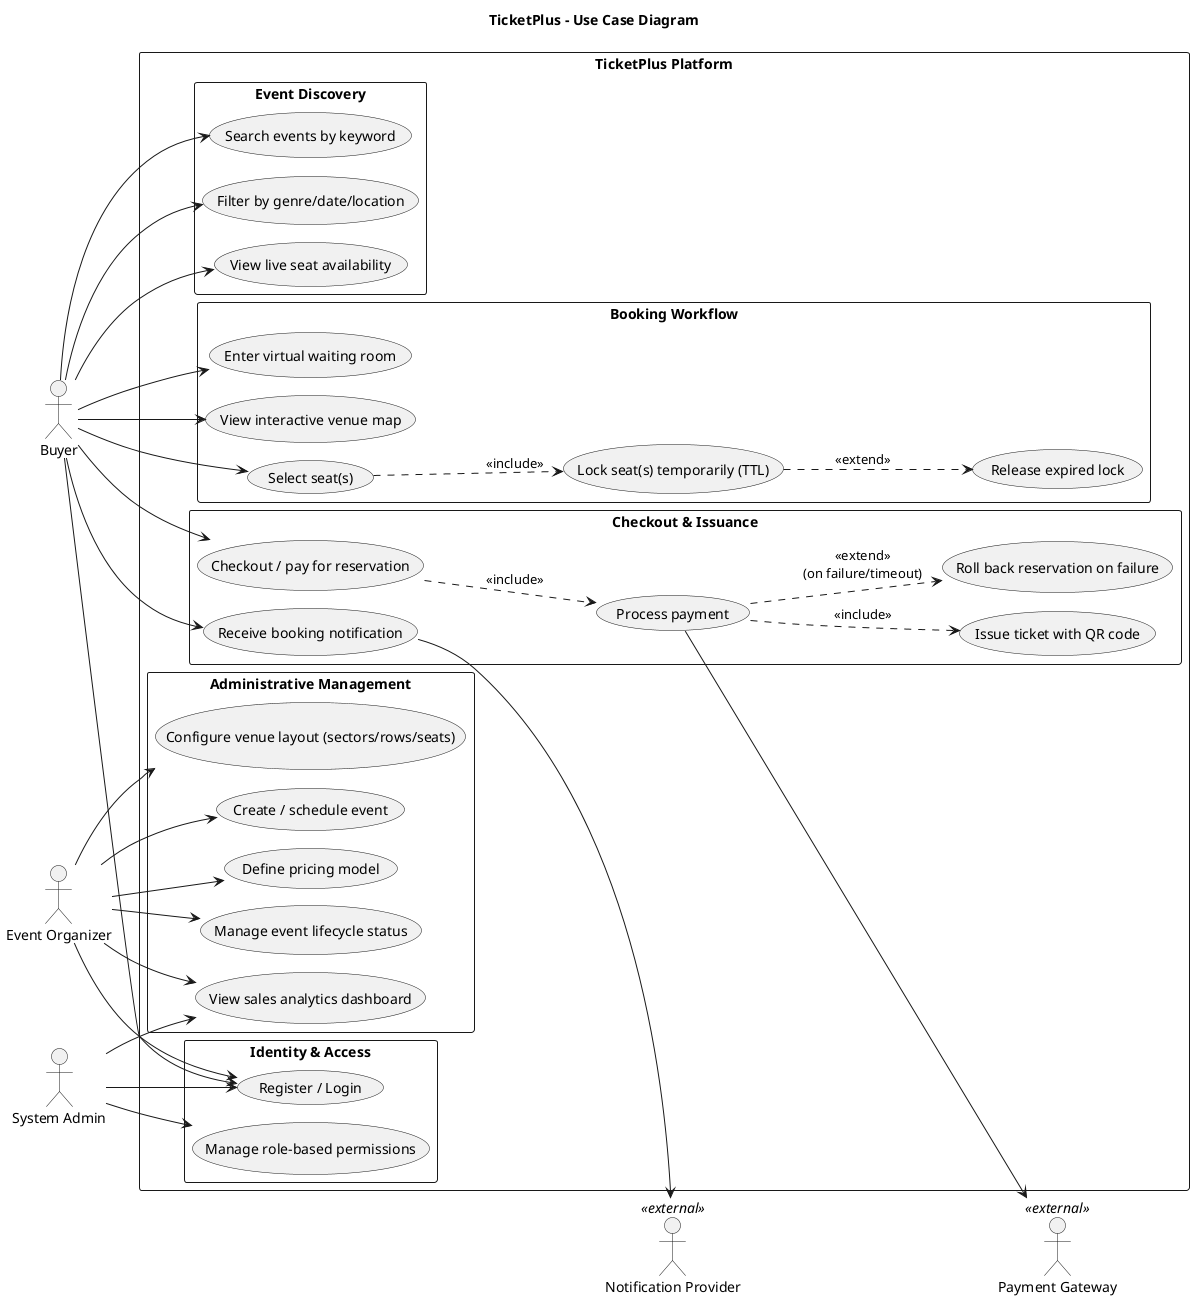
\includegraphics[width=0.94\textwidth,height=0.72\textheight,keepaspectratio]{figures/01-use-case.png}
\caption{نمودار موارد کاربرد تیکت‌پلاس}
\end{figure}

\subsection{نمودار کلاس}
مدل دامنه شامل کاربر، برگزارکننده، رویداد، سالن، بخش، ردیف، صندلی، قانون قیمت،
رزرو، پرداخت، بلیت و اعلان است. وضعیت رزرو و پرداخت صریح مدل شده و زمان انقضا و
کلید تکرارپذیری در موجودیت رزرو قرار دارد.
\begin{figure}[H]
\centering
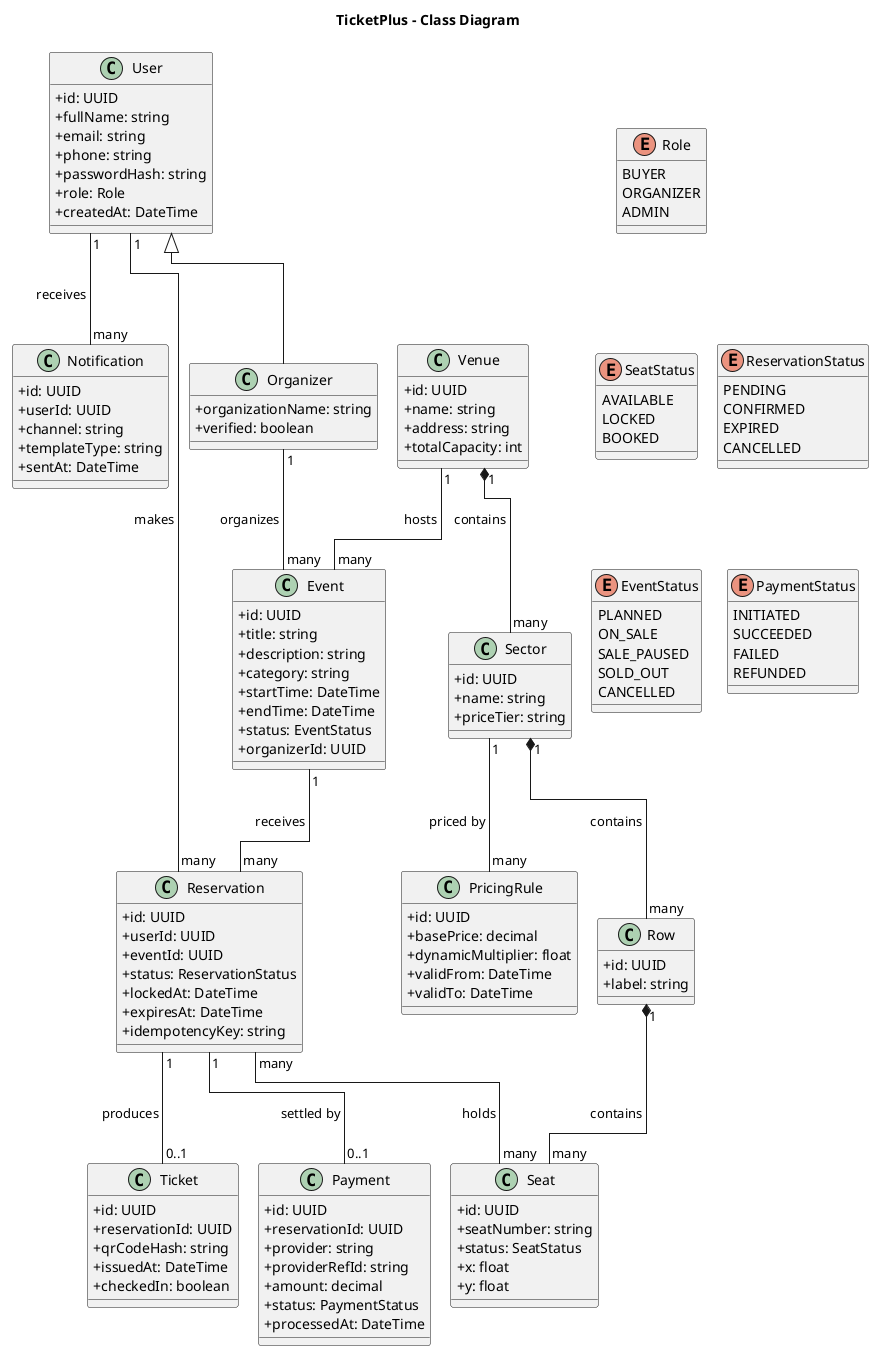
\includegraphics[width=0.96\textwidth,height=0.78\textheight,keepaspectratio]{figures/02-class-diagram.png}
\caption{نمودار کلاس‌های اصلی دامنه}
\end{figure}

\subsection{نمودارهای توالی}
توالی خرید، ورود اختیاری به اتاق انتظار، قفل اتمیک، ثبت رزرو، فراخوانی درگاه،
تأیید یا جبران و صدور مستقل بلیت را نشان می‌دهد. در شکست پرداخت، رزرو لغو و
صندلی آزاد می‌شود. در انقضای بدون پرداخت نیز کلید قفل حذف و وضعیت رزرو منقضی
می‌شود.
\begin{figure}[H]
\centering
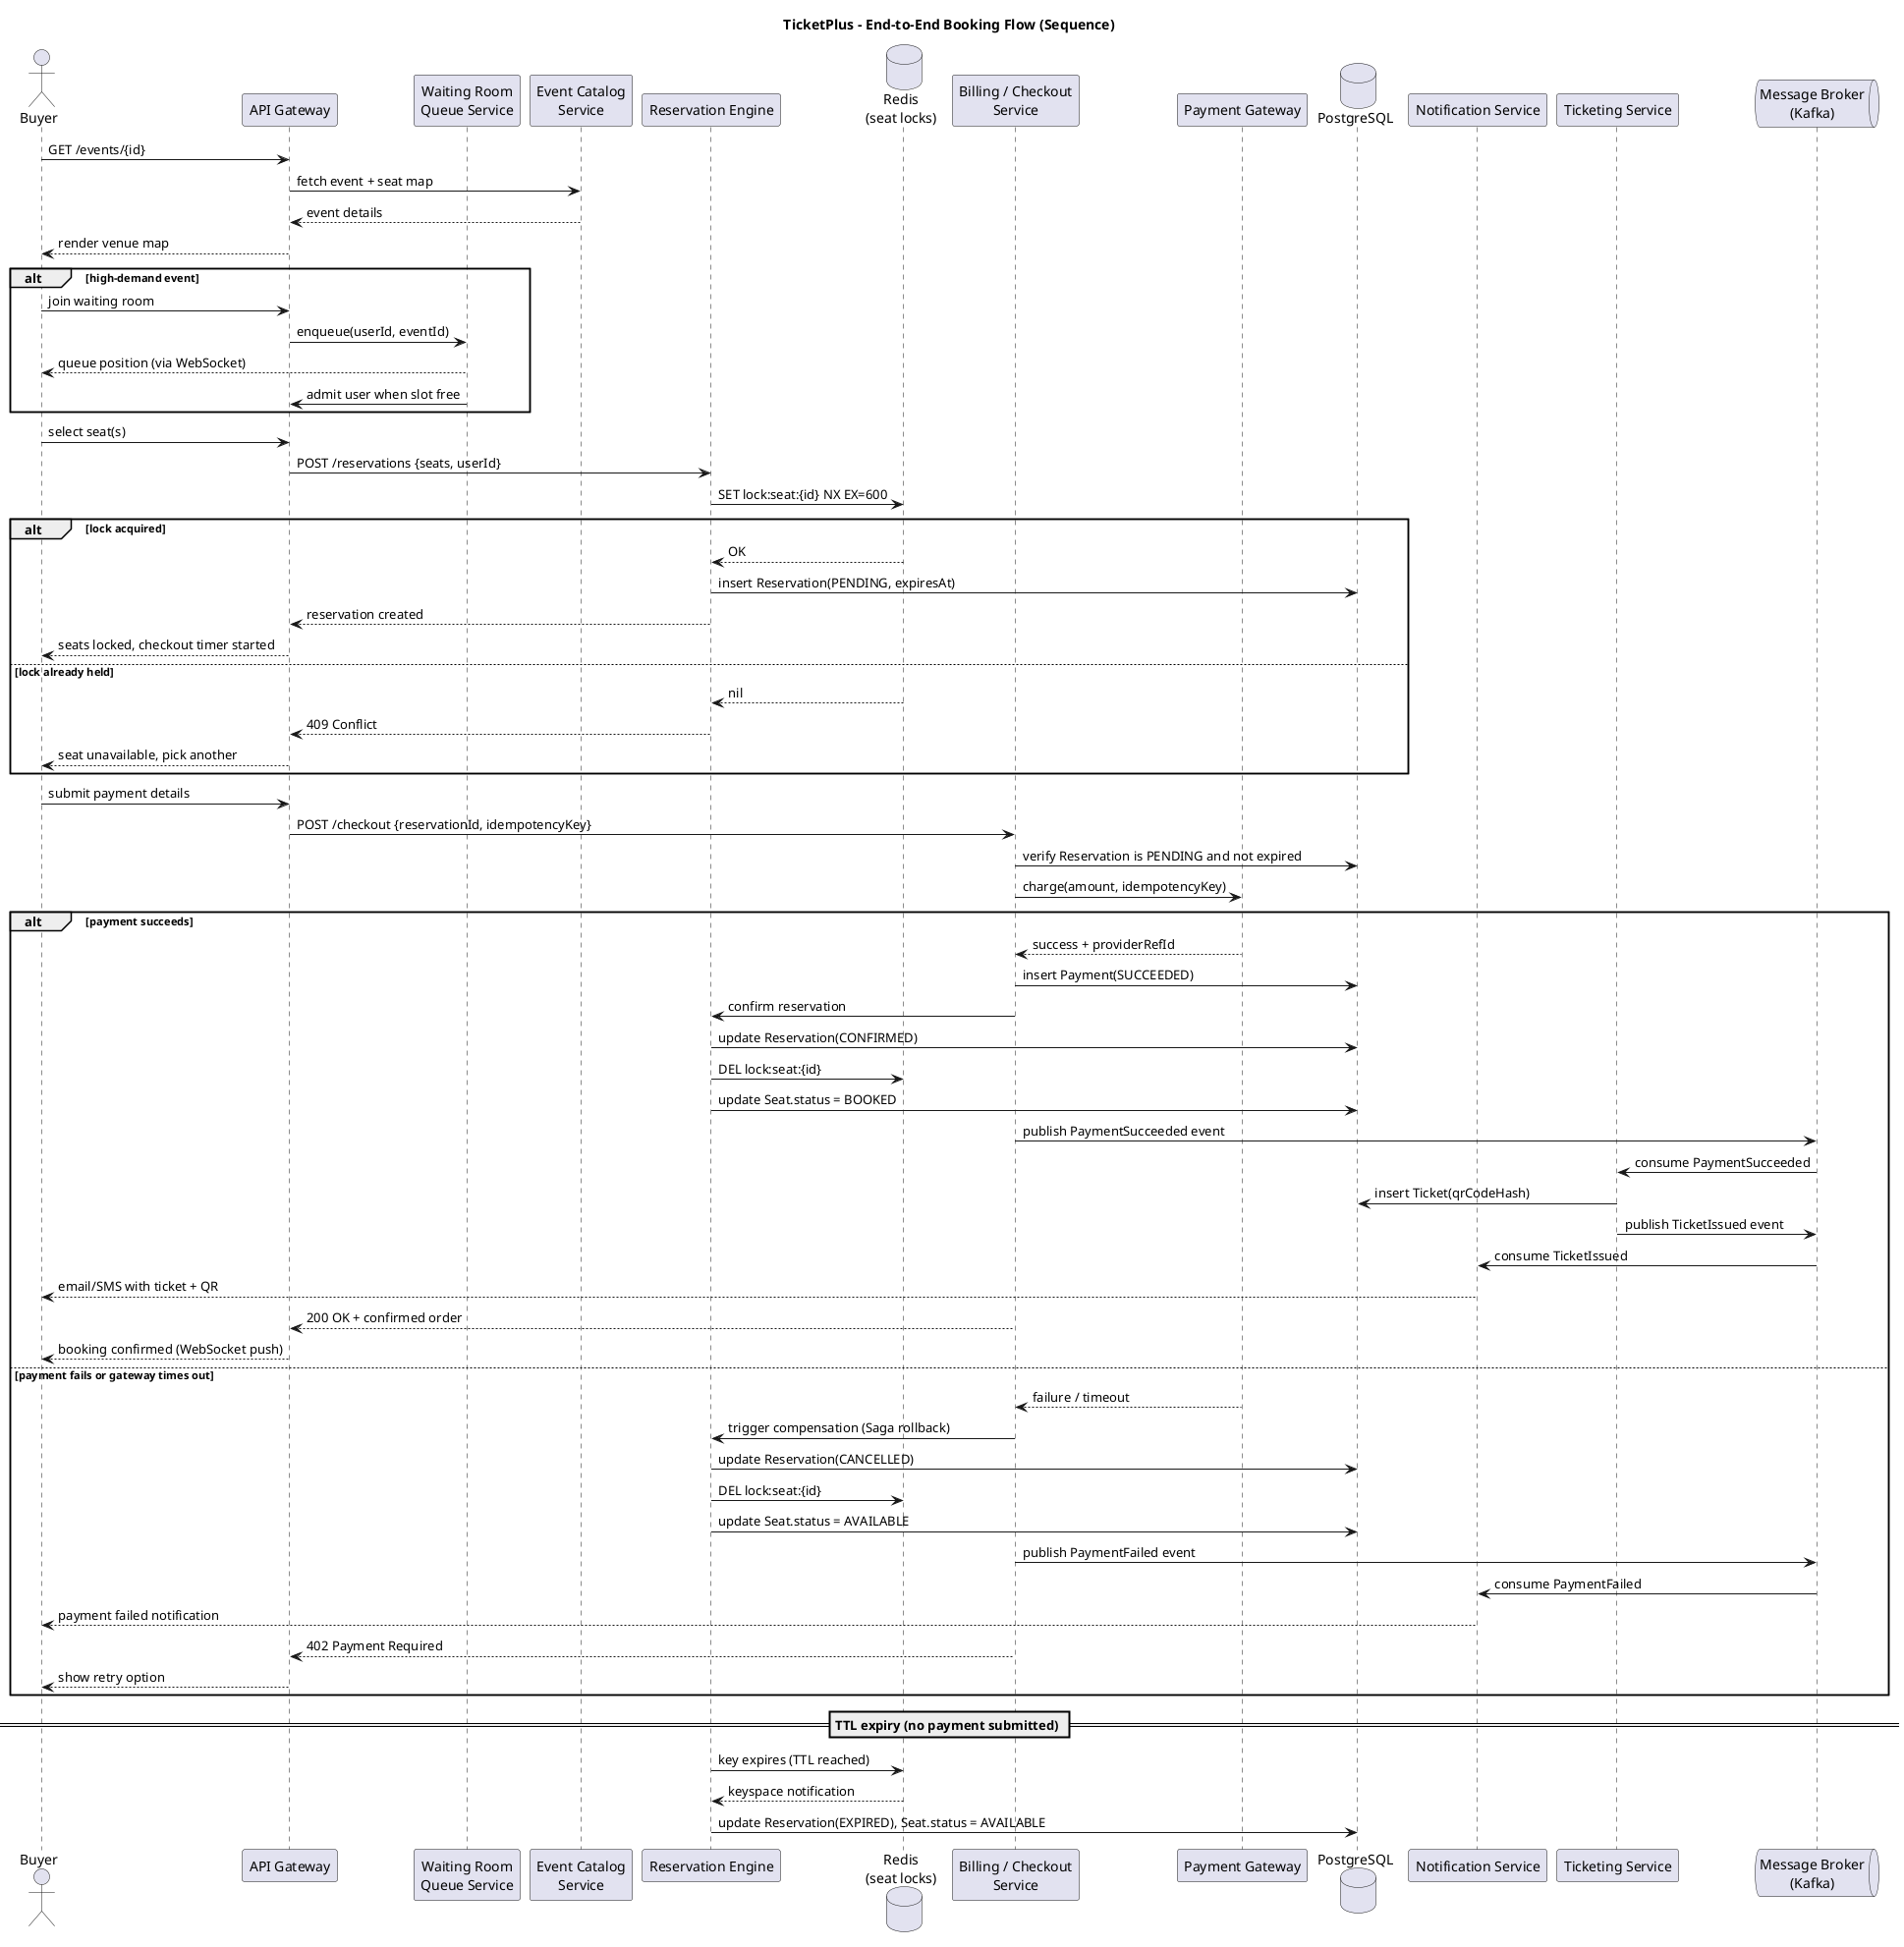
\includegraphics[width=0.96\textwidth,height=0.82\textheight,keepaspectratio]{figures/03-sequence-booking-flow.png}
\caption{توالی انتهابه‌انتهای خرید بلیت}
\end{figure}

جریان اعلان از طریق کافکا از پرداخت جدا شده است. سرویس بلیت رویداد موفقیت
پرداخت را مصرف می‌کند، بلیت را می‌سازد و رویداد صدور بلیت را برای اعلان منتشر
می‌کند.
\begin{figure}[H]
\centering
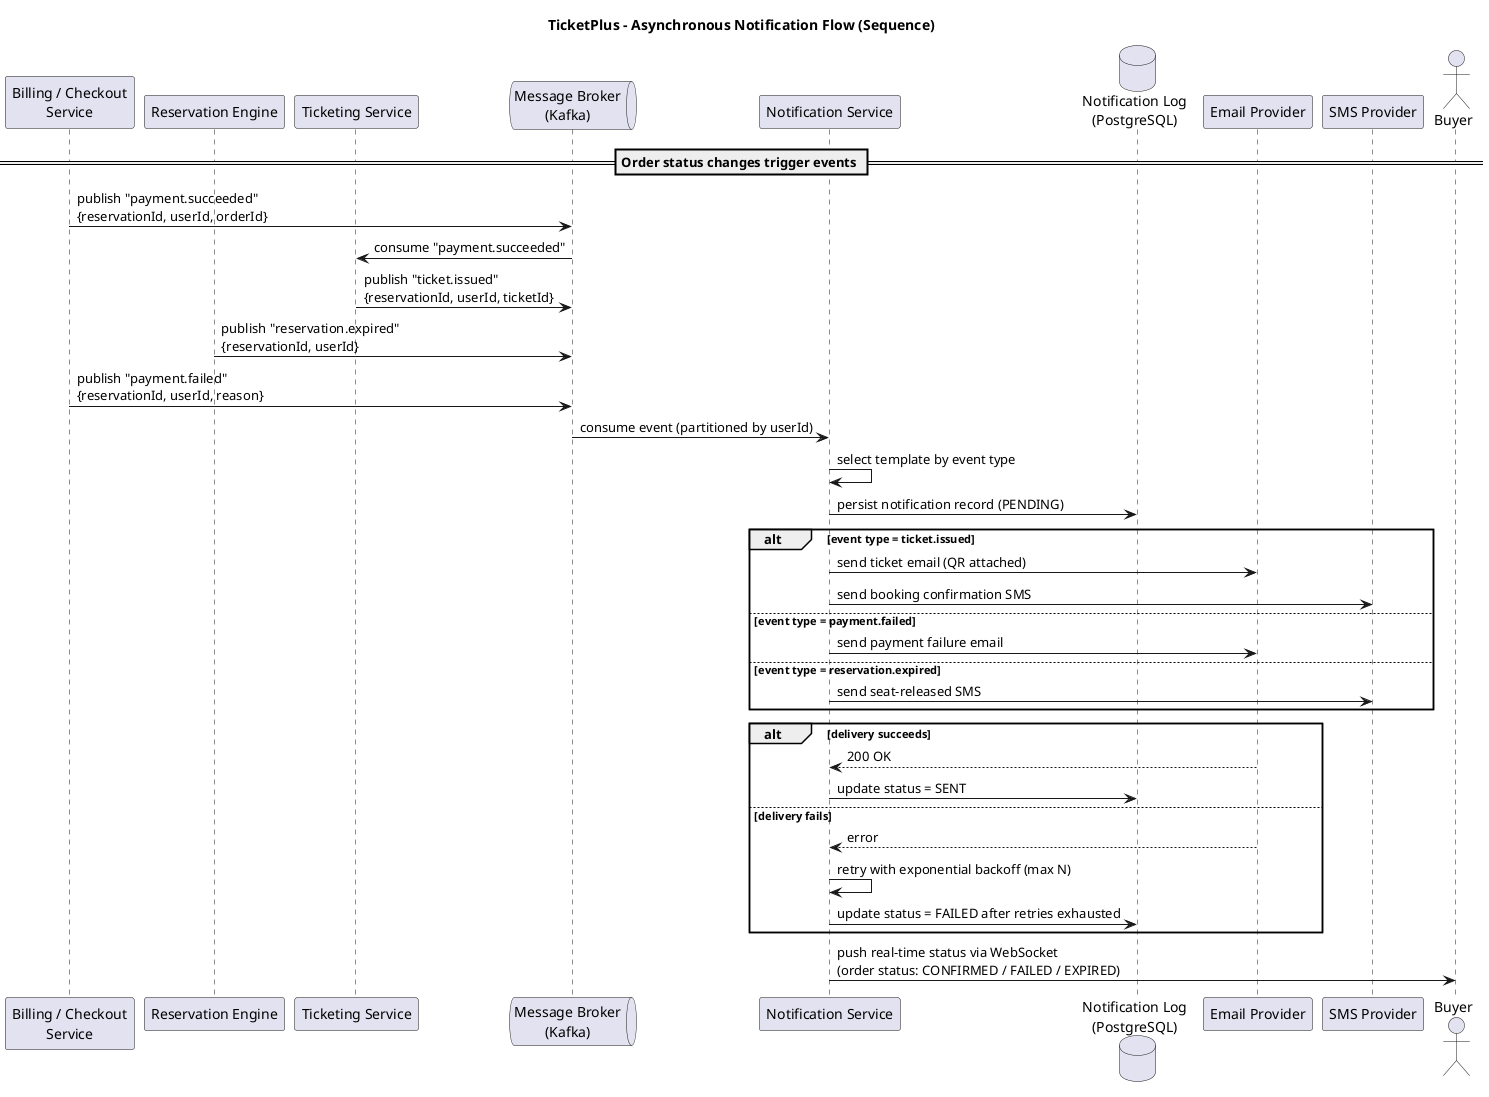
\includegraphics[width=0.95\textwidth,height=0.75\textheight,keepaspectratio]{figures/04-sequence-notification-flow.png}
\caption{توالی اعلان و صدور غیرهم‌زمان بلیت}
\end{figure}

\subsection{نمودارهای فعالیت}
مسیر فعالیت خریدار، شاخه‌های رقابت صندلی، انقضای زمان، شکست پرداخت و خرید موفق
را پوشش می‌دهد. فعالیت برگزارکننده نیز ایجاد سالن، تعریف قیمت، اعتبارسنجی،
انتشار و پایش فروش را مدل می‌کند.
\begin{figure}[H]
\centering
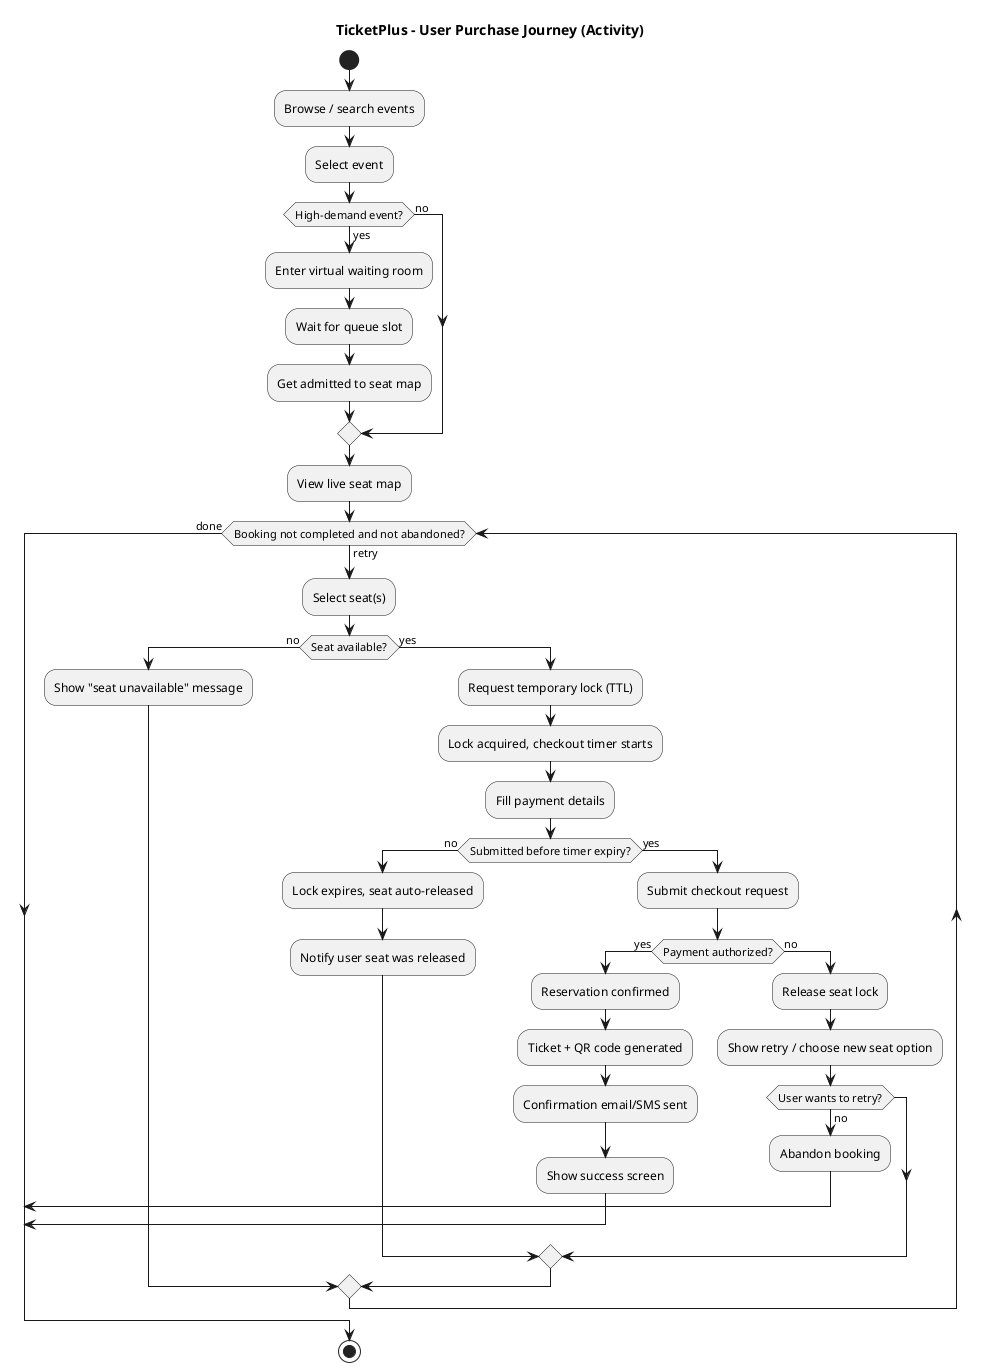
\includegraphics[width=0.88\textwidth,height=0.72\textheight,keepaspectratio]{figures/05-activity-user-purchase.png}
\caption{فعالیت خرید کاربر}
\end{figure}
\begin{figure}[H]
\centering
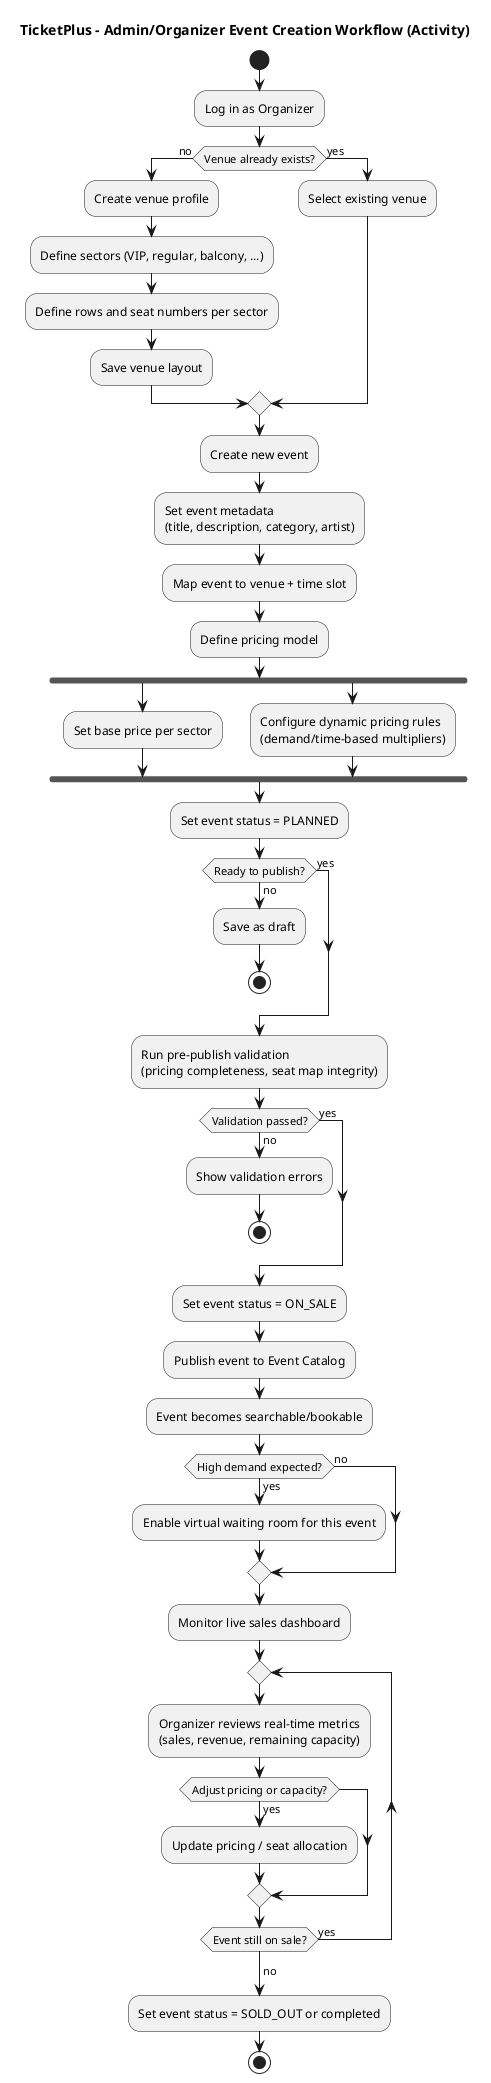
\includegraphics[width=0.88\textwidth,height=0.72\textheight,keepaspectratio]{figures/06-activity-admin-event-creation.png}
\caption{فعالیت ایجاد و انتشار رویداد}
\end{figure}

\subsection{معماری مؤلفه‌ای}
مرزهای مستقل شامل درگاه API، هویت، کاتالوگ، اتاق انتظار، رزرو، پرداخت، بلیت و
اعلان هستند. پایگاه داده هر حوزه به صورت منطقی خصوصی است. سرویس بلیت مالک چرخه
صدور و اعتبارسنجی است و دیگر در حوزه پرداخت قرار ندارد.
\begin{figure}[H]
\centering
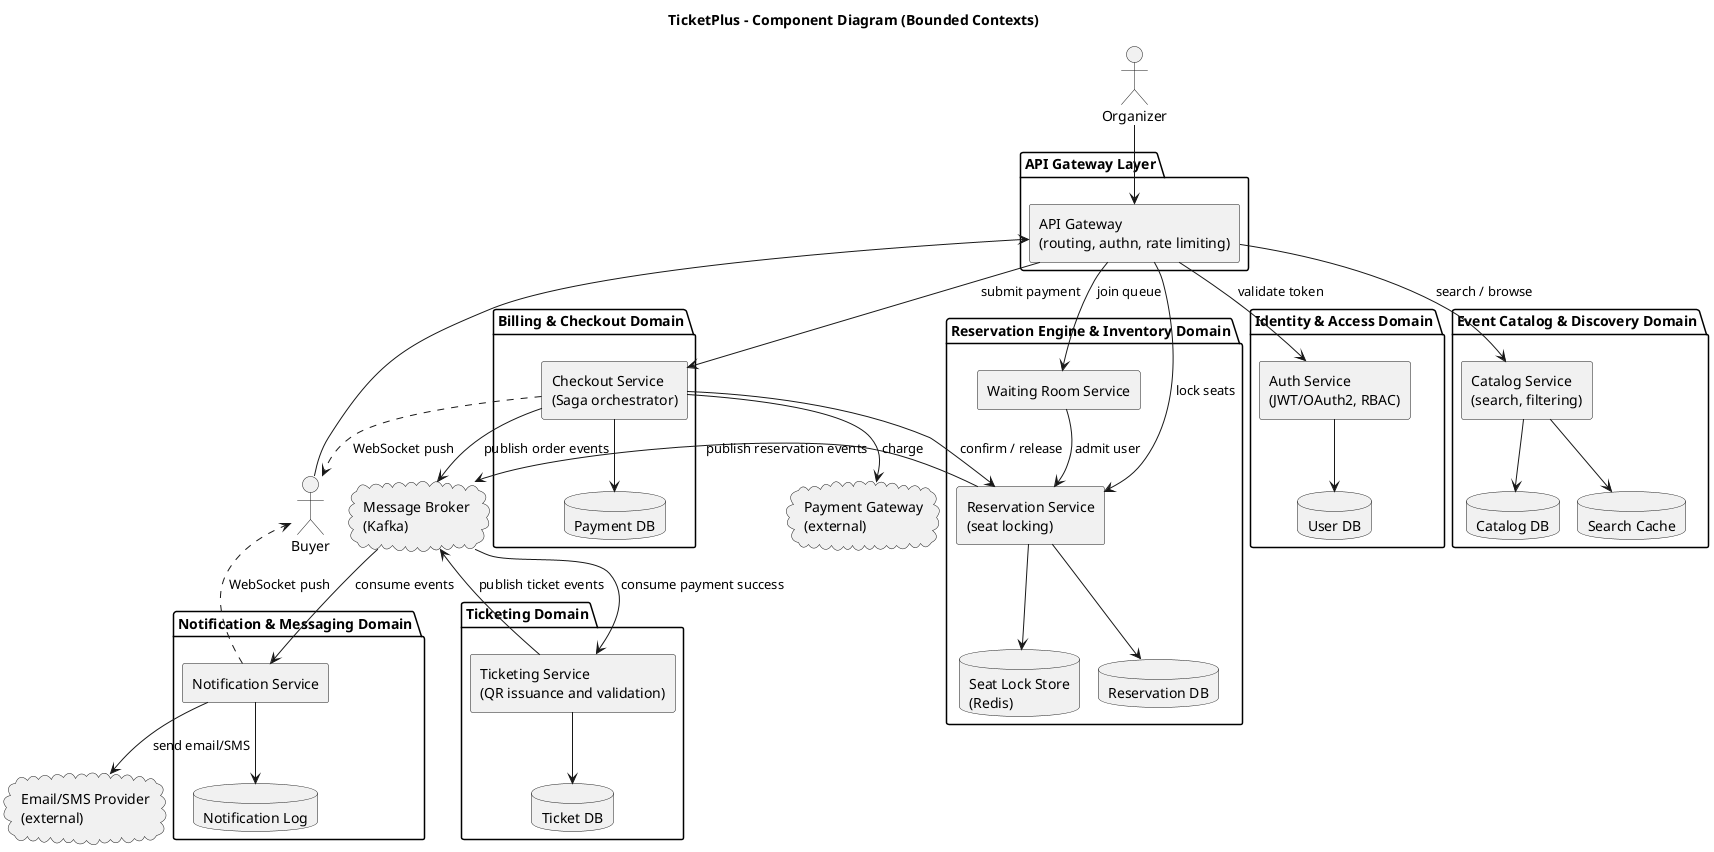
\includegraphics[width=0.98\textwidth,height=0.78\textheight,keepaspectratio]{figures/07-component-diagram.png}
\caption{نمودار مؤلفه‌ها و حوزه‌های سامانه}
\end{figure}

\subsection{معماری استقرار}
در استقرار تولید، ترافیک از بارمتوازن‌کننده و ورودی کوبرنتیز به درگاه API و
سپس سرویس‌ها هدایت می‌شود. پستگرس داده پایدار، ردیس قفل موقت و کافکا رویدادهای
غیرهم‌زمان را نگهداری می‌کنند. پرومتئوس و گرافانا برای پایش استفاده می‌شوند.
\begin{figure}[H]
\centering
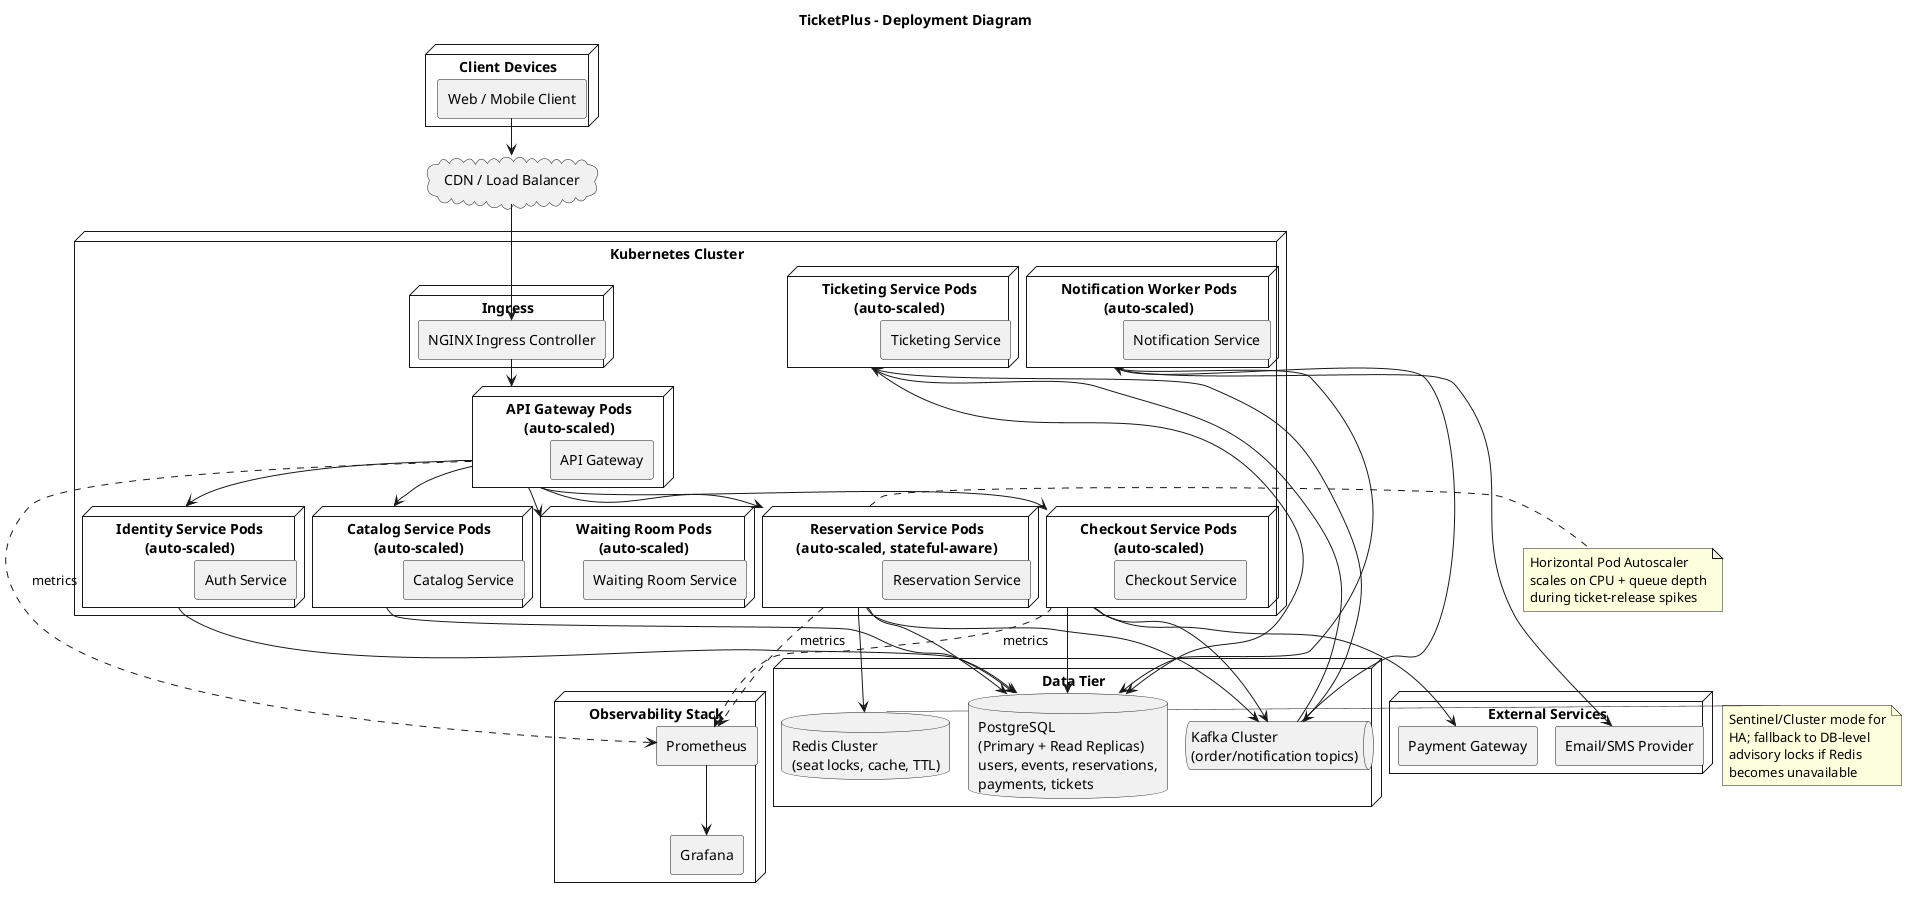
\includegraphics[width=0.98\textwidth,height=0.80\textheight,keepaspectratio]{figures/08-deployment-diagram.png}
\caption{نمودار استقرار تولید}
\end{figure}

\section{معماری تولید و عملیات}

\subsection{مرزبندی حوزه‌ها}
تصمیم اصلی طراحی این است که هندسه سالن در کاتالوگ، اما وضعیت زنده صندلی در
رزرو نگهداری شود. کاتالوگ فقط projection موجودی را برای جست‌وجو مصرف می‌کند و
هرگز وضعیت قفل را نمی‌نویسد. این تصمیم وابستگی حلقوی کاتالوگ و رزرو را حذف و
قاعده جلوگیری از overbooking را به یک مالک واگذار می‌کند.
\begin{figure}[H]
\centering
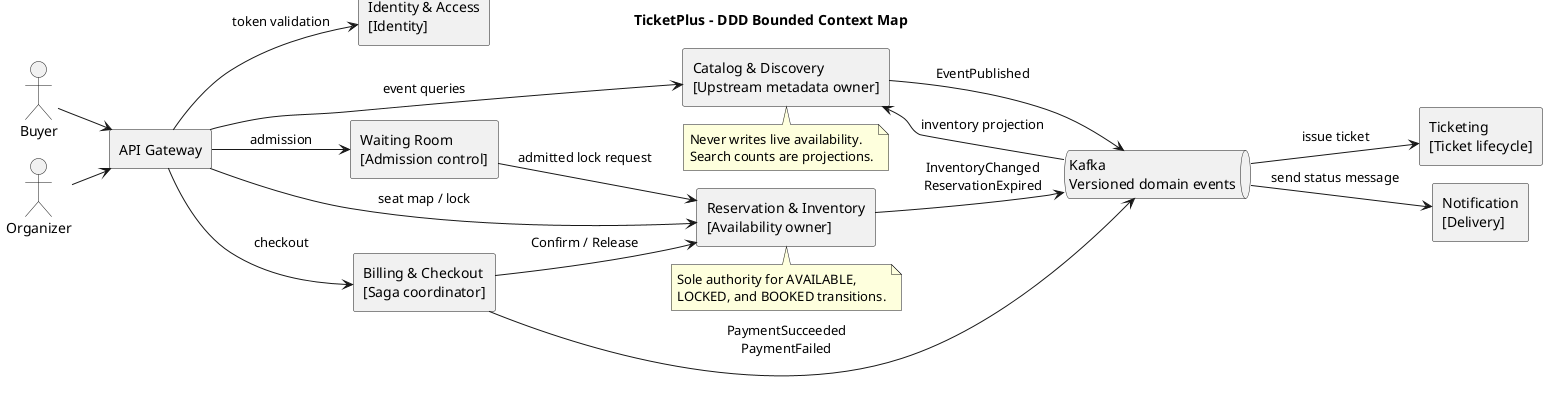
\includegraphics[width=0.96\textwidth,height=0.72\textheight,keepaspectratio]{figures/bounded-context-map.png}
\caption{نقشه حوزه‌های محدودشده}
\end{figure}

\subsection{پیام‌رسانی غیرهم‌زمان}
تغییر وضعیت کسب‌وکار همراه رکورد outbox در یک تراکنش ثبت می‌شود. relay رویداد
را در کافکا منتشر می‌کند. مصرف‌کنندگان شناسه رویداد پردازش‌شده را نگه می‌دارند،
در خطای موقت با backoff و jitter تکرار می‌کنند و پس از پنج شکست پیام را به
dead-letter queue انتقال می‌دهند. کلید پارتیشن شناسه رزرو یا سفارش است تا ترتیب
همان aggregate حفظ شود.
\begin{figure}[H]
\centering
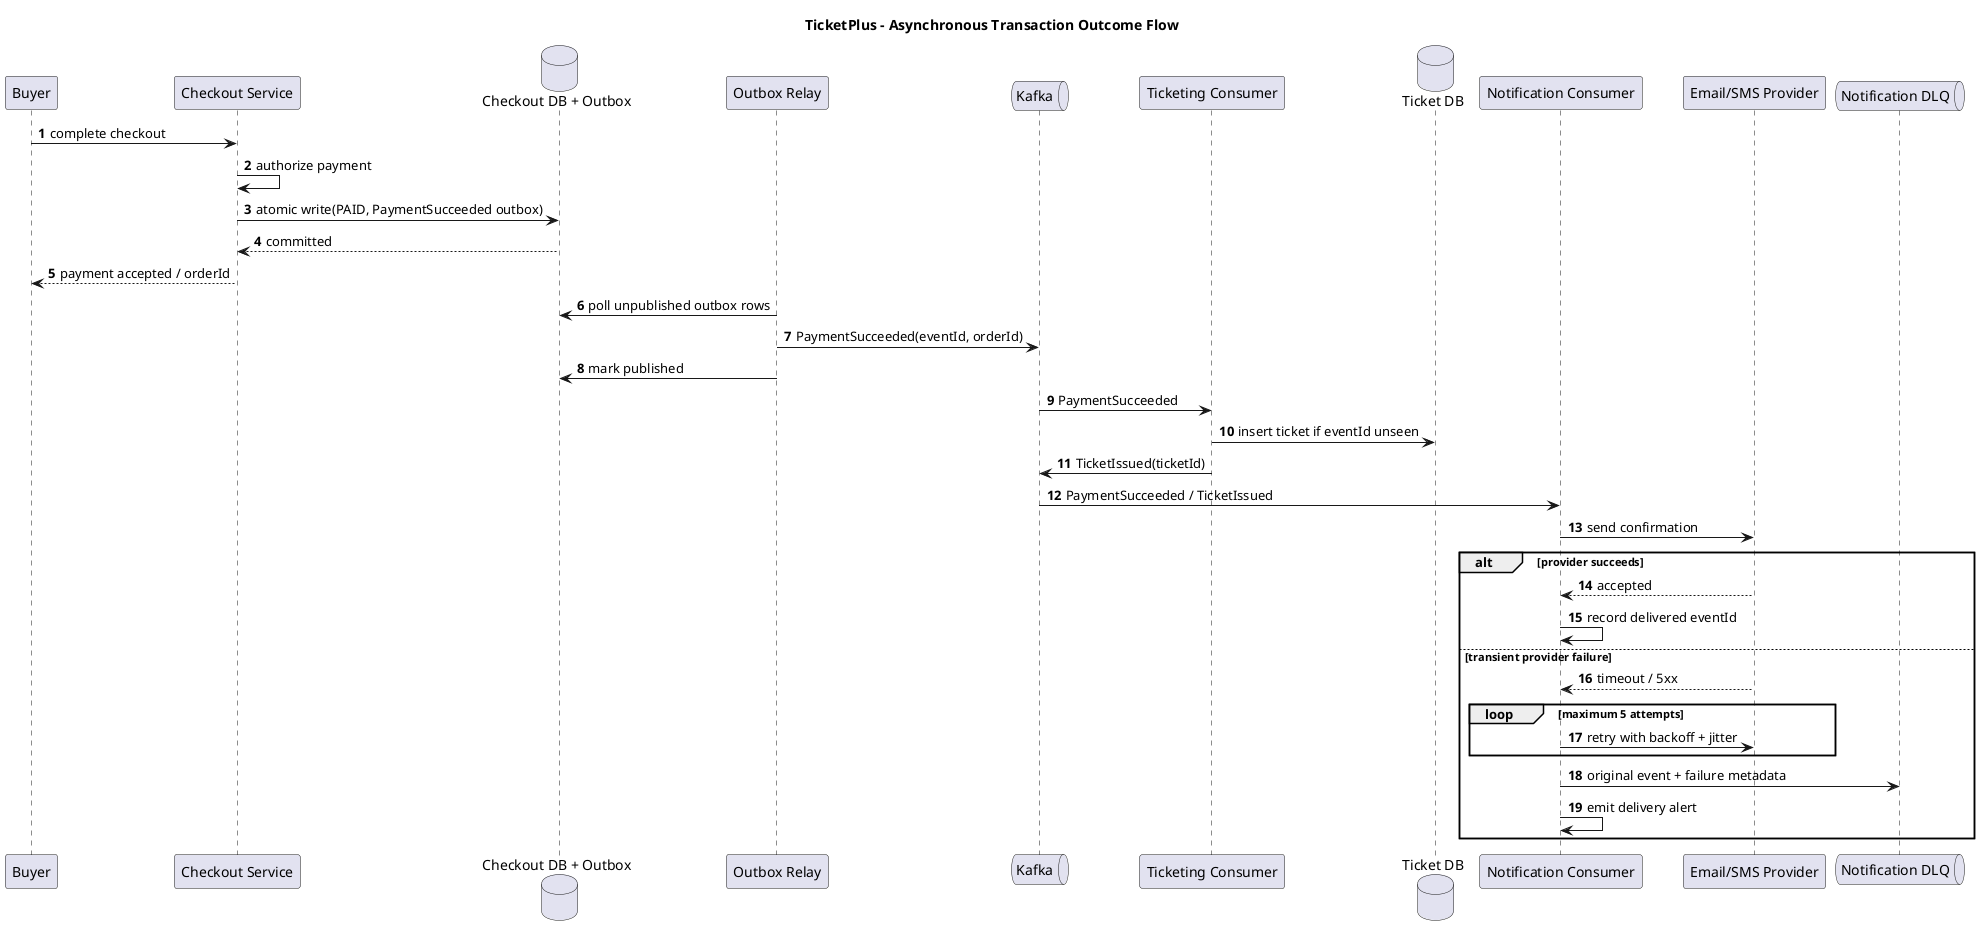
\includegraphics[width=0.96\textwidth,height=0.76\textheight,keepaspectratio]{figures/async-transaction-flow.png}
\caption{جریان غیرهم‌زمان نتیجه تراکنش}
\end{figure}

\subsection{پایش، SLO و انتشار Canary}
انتشار canary با ۵ درصد ترافیک آغاز و پس از پنجره‌های تحلیل به ۲۵، ۵۰ و ۱۰۰
درصد افزایش می‌یابد. عبور نرخ خطا، تأخیر یا conflict رزرو از نسخه پایدار، rollback
خودکار را فعال می‌کند. پرومتئوس معیارهای سرویس، ورودی، کوبرنتیز، کافکا، ردیس و
پستگرس را جمع و گرافانا نمایش می‌دهد. OpenTelemetry شناسه trace و correlation
را میان HTTP و پیام‌ها منتقل می‌کند.
\begin{figure}[H]
\centering
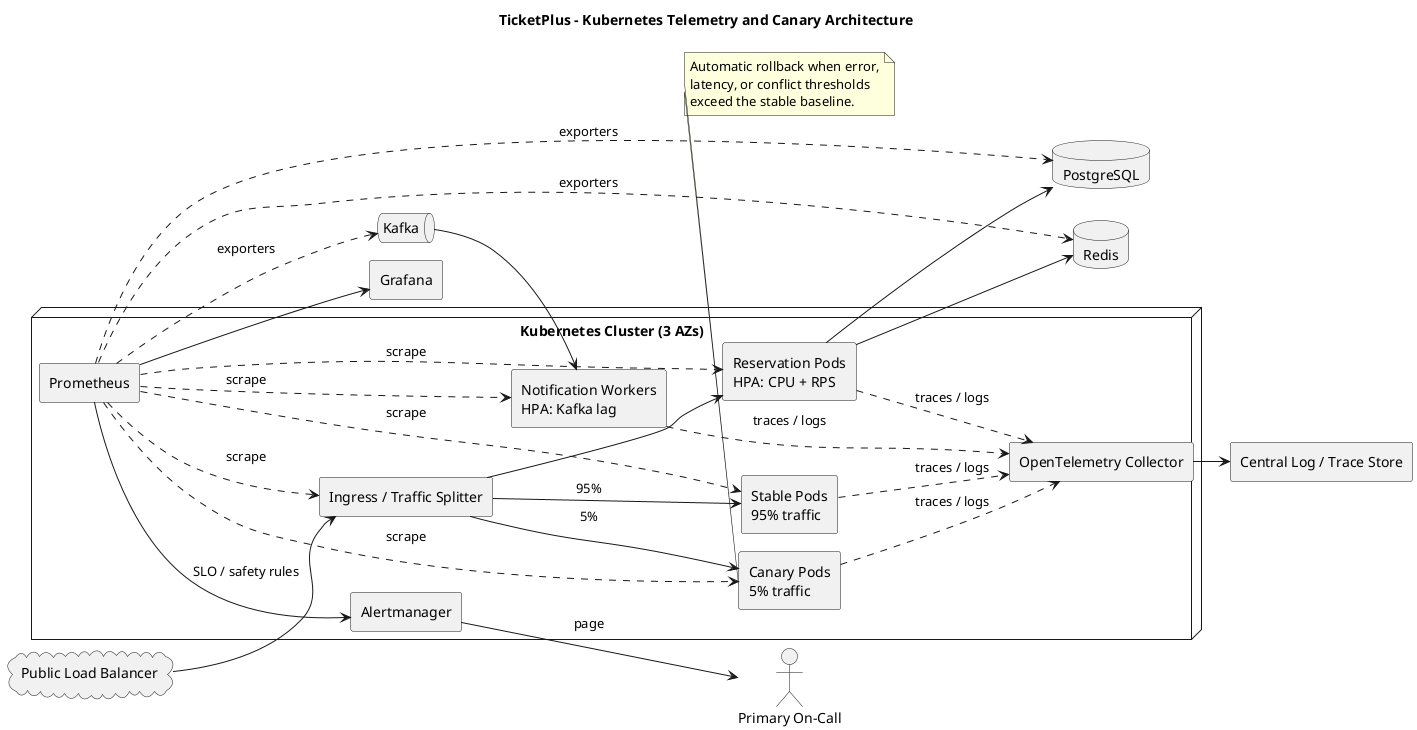
\includegraphics[width=0.96\textwidth,height=0.76\textheight,keepaspectratio]{figures/production-telemetry.png}
\caption{معماری مشاهده‌پذیری و انتشار Canary}
\end{figure}

اهداف اصلی شامل دسترس‌پذیری ۹۹٫۹۵ درصد برای قفل و پرداخت، صدک ۹۵ قفل کمتر از
۳۰۰ میلی‌ثانیه، lag کافکا کمتر از ۳۰ ثانیه و صفر رزرو مضاعف است. هر نشانه رزرو
مضاعف بلافاصله رخداد سطح یک ایجاد می‌کند.

\subsection{مدیریت رخداد}
شدت رخداد از \term{SEV-1} تا \term{SEV-4} تعریف شده است. فرمانده رخداد تصمیم و
اولویت، مسئول عملیات اقدام فنی، مسئول ارتباطات اطلاع‌رسانی و نویسنده timeline
را نگهداری می‌کند. on-call اولیه و ثانویه هفتگی هستند و عدم پاسخ در پنج دقیقه
به جانشین escalation می‌شود. پایان رخداد نیازمند پایداری SLO برای ۳۰ دقیقه،
تخلیه backlog و تطبیق رزرو، پرداخت و بلیت است.

\subsection{پسامورتوم‌های اجباری}
سه تحلیل بدون سرزنش تهیه شده است:
\begin{enumerate}
  \item خرابی درگاه پرداخت و باقی ماندن صندلی‌ها در حالت قفل؛ راه‌حل شامل circuit
  breaker، تطبیق با کلید تکرارپذیری و تأیید، آزادسازی یا قرنطینه سفارش است.
  \item شکست worker اتاق انتظار زیر بار شدید و پاسخ 503؛ راه‌حل شامل صف پایدار،
  حفظ توکن کاربر، حالت FIFO تنزل‌یافته و retry دارای jitter است.
  \item پارتیشن شبکه بین درگاه و رزرو؛ سامانه خرید را fail-closed می‌کند، policy
  معیوب را rollback و پس از بازیابی تطبیق انجام می‌دهد.
\end{enumerate}
هر پسامورتوم اثر، timeline، علت ریشه‌ای، عوامل تشدیدکننده، رفع و اقدام اصلاحی
دارای مالک و موعد را ثبت می‌کند.

\section{زیرساخت و استقرار خودکار}

زیرساخت ابری به‌صورت اعلامی در مسیر \en{infra/terraform/} تعریف شده است.
منابع اصلی عبارت‌اند از شبکه چندناحیه‌ای، زیرشبکه عمومی و خصوصی، دروازه اینترنت، دروازه
\term{NAT}، خوشه \term{EKS}، گروه گره خودمقیاس، پایگاه داده \term{RDS
PostgreSQL} چندناحیه‌ای، ردیس مدیریت‌شده، کافکای مدیریت‌شده \term{MSK} و
بارمتوازن‌کننده کاربردی.

\begin{center}
\begin{tabular}{P{4cm}P{10cm}}
\toprule
فایل & مسئولیت\\
\midrule
\en{network.tf} & شبکه، زیرشبکه‌ها، مسیرها و دروازه‌های خروجی\\
\en{eks.tf} & خوشه کوبرنتیز و گروه گره خودمقیاس\\
\en{rds.tf} & پستگرس رمزگذاری‌شده، چندناحیه‌ای و نسخه خواندنی\\
\en{redis.tf} & قفل صندلی با تکرار، failover و رمزگذاری\\
\en{msk.tf} & کارگزاران کافکا، TLS و ثبت رخداد در CloudWatch\\
\en{loadbalancer.tf} & ALB عمومی، listener و target group ورودی\\
\en{variables.tf} و \en{outputs.tf} & پارامترهای محیط و خروجی‌های اتصال\\
\bottomrule
\end{tabular}
\end{center}

فرمت ترافورم با نسخه ۱٫۹٫۸ بررسی شد و اعمال منابع انجام نشد تا هزینه ابری
ایجاد نشود. اعتبارسنجی وابسته به provider در خط لوله گیت‌لب انجام می‌شود؛
registry محلی محیط فعلی پروتکل provider را ارائه نکرد.


\part{کیفیت، پیاده‌سازی و استانداردهای مهندسی}

\section{چرخه چابک، بازبینی و تضمین کیفیت}

\subsection{فرآیند توسعه و بازبینی}
قواعد مشارکت در \en{CONTRIBUTING.md} تعریف شده است. تغییرات با شاخه مرتبط با
شماره کار جیرا، merge request، آزمون، مستندات و تأیید مالک حوزه ادغام می‌شوند.
تغییرات رزرو، پرداخت، هویت، مهاجرت داده و زیرساخت به دو تأیید نیاز دارند. قالب
merge request شامل رفتار، شواهد آزمون، سازگاری قرارداد، مهاجرت، مشاهده‌پذیری و
روش rollback است.

\subsection{بخش رزروشده مدیریت چابک}
\reservedbox{خروجی جیرا و اسپرینت‌ها}{تصاویر یا خروجی‌های backlog، epic، story،
task، برنامه‌ریزی اسپرینت، burndown chart، sprint review و retrospective واقعی
گروه در این قسمت قرار گیرد. برای هر تصویر شماره اسپرینت و بازه زمانی نوشته شود.}

\reservedbox{شواهد بازبینی کد}{در صورت نیاز، نمونه merge request، نظرهای
بازبین‌ها، نتیجه pipeline و تصمیم ادغام واقعی گروه در این قسمت افزوده شود.}

\subsection{راهبرد آزمون}
اولویت آزمون ابتدا صحت خرید، سپس دسترس‌پذیری، امنیت، کارایی و نگهداشت‌پذیری
است. برای ماژول رزرو حداقل پوشش خط ۹۰ درصد و شاخه ۸۵ درصد و برای منطق حیاتی
امتیاز جهش حداقل ۸۵ درصد تعیین شد. هیچ استثنایی برای رزرو مضاعف، پرداخت تکراری،
دور زدن مجوز یا از دست رفتن غیرقابل بازیابی داده پذیرفته نمی‌شود.

اوراکل صحت پس از آزمون هم‌زمانی بررسی می‌کند که هر صندلی رویداد حداکثر یک رزرو
تأییدشده داشته باشد، هر صندلی فروخته‌شده دقیقاً یک مالک داشته باشد، پرداخت موفق
به سفارش تأییدشده یا بازپرداخت صریح متصل باشد و رزرو منقضی قفل زنده باقی
نگذارد.

\subsection{آزمون‌های پیاده‌سازی‌شده}
پیاده‌سازی مرجع با چارچوب استاندارد \term{unittest} آزموده شد و به نصب بسته
خارجی نیاز ندارد.

\begin{center}
\begin{tabular}{P{7.5cm}C{2.2cm}P{4.2cm}}
\toprule
سناریو & وضعیت & نتیجه\\
\midrule
رقابت ۲۰۰ درخواست هم‌زمان برای یک صندلی & موفق & دقیقاً یک برنده\\
تکرار درخواست رزرو با کلید یکسان & موفق & شناسه رزرو یکسان\\
ورودی دارای صندلی تکراری & موفق & رد ورودی\\
انقضا و رزرو مجدد صندلی & موفق & آزادسازی صحیح\\
تأیید دقیقاً در مرز انقضا & موفق & رد و ثبت انقضا\\
پرداخت موفق و صدور بلیت & موفق & تأیید رزرو و یک بلیت\\
پرداخت شکست‌خورده & موفق & جبران و آزادسازی\\
پرداخت با نتیجه نامشخص & موفق & نگهداری برای تطبیق\\
تحویل تکراری رویداد پرداخت & موفق & عدم صدور بلیت دوم\\
آزمون HTTP انتهابه‌انتها & مشروط & در sandbox به علت منع socket رد شد؛ در CI اجرا می‌شود\\
\bottomrule
\end{tabular}
\end{center}

\subsection{پوشش و آزمون جهش}
ابزار پوشش مستقل پروژه، دستورات قابل اجرای ماژول‌های رزرو، پرداخت و رویداد را
با AST پایتون و trace زمان اجرا مقایسه می‌کند. نتیجه آخرین اجرا در جدول زیر است.

\begin{center}
\begin{tabular}{P{5cm}C{3cm}C{3cm}C{2.5cm}}
\toprule
ماژول & دستورات قابل اجرا & دستورات پوشش‌یافته & درصد\\
\midrule
\en{reservation.py} & ۱۰۸ & ۹۶ & ۸۸٫۸۹\\
\en{checkout.py} & ۶۱ & ۶۰ & ۹۸٫۳۶\\
\en{events.py} & ۳۳ & ۳۲ & ۹۶٫۹۷\\
مجموع & ۲۰۲ & ۱۸۸ & ۹۳٫۰۷\\
\bottomrule
\end{tabular}
\end{center}

شش جهش حیاتی شامل پذیرش صندلی تکراری، حذف یکتایی مالک فعال، مجاز کردن تأیید در
مرز انقضا، وارونگی موفقیت پرداخت، حذف جبران شکست و حذف تکرارناپذیری صدور بلیت
اعمال شد. همه شش جهش توسط آزمون‌ها کشته شدند و امتیاز جهش ۱۰۰ درصد به دست آمد.

\subsection{آزمون بار و تنش}
اسکریپت \en{quality/load/hot-seat-contention.js} با \term{k6} به طور پیش‌فرض
۵۰۰۰ کاربر مجازی را برای قفل یک صندلی رقابت می‌دهد. معیار پذیرش دقیقاً یک پاسخ
موفق، conflictهای مورد انتظار، خطای فنی کمتر از یک درصد و صدک ۹۵ کمتر از ۷۵۰
میلی‌ثانیه است. برنامه کامل آزمون شامل هجوم لحظه‌ای، بار گسترده رزرو، اوج
پرداخت، soak هشت‌ساعته، spike و تزریق خرابی ردیس، کافکا، درگاه و شبکه است.

\subsection{خط لوله گیت‌لب}
خط لوله \en{.gitlab-ci.yml} مراحل زیر را اجرا می‌کند:
\begin{itemize}
  \item بررسی Markdown و لینک‌ها؛
  \item اعتبارسنجی و بازتولید PlantUML؛
  \item فرمت، init و validate ترافورم بدون backend؛
  \item آزمون، پوشش و جهش پیاده‌سازی مرجع؛
  \item اسکن آسیب‌پذیری، secret و misconfiguration با Trivy؛
  \item اجرای اختیاری آزمون k6 در محیط ایزوله؛
  \item ایجاد فایل ZIP در tag انتشار.
\end{itemize}

\section{پیاده‌سازی مرجع و قراردادها}

\subsection{ساختار کد}
پیاده‌سازی مرجع در \en{src/ticketplus/} و با کتابخانه استاندارد پایتون ۳٫۱۳
نوشته شده است. هدف آن اثبات قواعد حیاتی بدون تحمیل وابستگی حجیم به محیط توسعه
است.
\begin{center}
\begin{tabular}{P{4cm}P{10cm}}
\toprule
ماژول & مسئولیت\\
\midrule
\en{reservation.py} & تراکنش SQLite، قفل چندصندلی، انقضا، تأیید و آزادسازی\\
\en{checkout.py} & ساگای پرداخت، جبران، صدور بلیت و ثبت اعلان\\
\en{events.py} & گذرگاه رویداد محلی و مصرف تکرارناپذیر\\
\en{http_api.py} & آداپتور HTTP بدون وابستگی و endpointهای سلامت، رزرو، پرداخت و بلیت\\
\bottomrule
\end{tabular}
\end{center}

مهاجرت‌های پستگرس در \en{db/migrations/} schemaهای هویت، کاتالوگ، رزرو، پرداخت،
بلیت و اعلان را جدا می‌کنند. قید یکتایی مالک فعال در سطح دیتابیس نیز اعمال شده
است. جدول outbox برای انتشار پایدار رویدادها در نظر گرفته شده است.

\subsection{قرارداد API و رویداد}
فایل \en{contracts/openapi/ticketplus.yaml} قرارداد \term{OpenAPI 3.1} را برای
سلامت، ایجاد و دریافت رزرو، checkout و دریافت بلیت تعریف می‌کند. قراردادها
کلید Idempotency، ساختار مبلغ در واحد خرد و کدهای ۲۰۱، ۴۰۰، ۴۰۴ و ۴۰۹ را مشخص
می‌کنند. schemaهای JSON رویدادهای \term{PaymentSucceeded} و
\term{TicketIssued} شامل نسخه، شناسه aggregate، زمان و payload بدون داده کارت
هستند.

\subsection{اجرای محلی و بسته‌بندی}
فایل \en{Dockerfile} برنامه را با کاربر غیر root اجرا می‌کند. Compose پیش‌فرض
API مرجع و حجم پایدار SQLite را اجرا می‌کند. profile با نام
\en{production-parity} پستگرس، ردیس و کافکا را نیز بالا می‌آورد.

\begin{latin}
\begin{lstlisting}[language=bash]
docker compose up --build
curl http://localhost:8080/health/ready

docker compose --profile production-parity up --build

PYTHONPATH=src python3 -m unittest discover -s tests -v
python3 quality/coverage/run.py
python3 quality/mutation/run.py
\end{lstlisting}
\end{latin}

اسکریپت \en{scripts/package-submission.sh} فایل ZIP را بدون metadata گیت، state
ترافورم، cache و bytecode می‌سازد. صحت استخراج آرشیو آزمایشی نیز بررسی شد.

\section{استانداردهای مهندسی و نقش‌های تیم}

هر سرویس تولیدی باید dependency قفل‌شده، container چندمرحله‌ای، endpointهای
سلامت، log ساختاریافته، معیار پرومتئوس، قرارداد نسخه‌دار، مهاجرت سازگار، آزمون
و runbook داشته باشد. داده کارت ذخیره نمی‌شود و secret در مخزن یا log قرار
نمی‌گیرد. تغییر قرارداد شکستن‌پذیر نیازمند نسخه جدید و بازه مهاجرت است.

دیدگاه‌های شبیه‌سازی‌شده شامل مالک محصول، تحلیلگر سیستم، توسعه‌دهنده backend و
frontend، متخصص QA، مهندس DevOps/SRE، بازبین امنیت و فرمانده رخداد است. ماتریس
مسئولیت، شخص پاسخگو، مشاوران و افراد مطلع را برای محدوده، قرارداد، رزرو، پرداخت،
آزمون، زیرساخت، رخداد و انتشار مشخص می‌کند.

برای دفاع معماری، اعضا باید بتوانند تصمیم مالکیت موجودی، ترکیب ردیس و قید
دیتابیس، انتخاب ساگا به‌جای تراکنش توزیع‌شده و سازگاری نهایی جست‌وجو را توضیح
دهند. تحویل حداقل یک‌بار کافکا، انتشار \term{Canary}، نتیجه آزمون رقابتی و
محدودیت تک‌منطقه‌ای نیز باید قابل دفاع باشند.


\part{جمع‌بندی، پیوست‌ها و مراجع مخزن}

\section{موارد باقی‌مانده برای نسخه تحویلی گروه}

سند چشم‌انداز محصول (بخش \ref{sec:vision})، سند تحلیل و کاهش ریسک (بخش
\ref{sec:risk}) و تحلیل رقابتی بازار اکنون در این گزارش تکمیل شده‌اند. بخش‌های
زیر همچنان عمداً توسط این گزارش جعل یا تکمیل فرض نشده‌اند و باید با شواهد
واقعی گروه جایگزین شوند:

\begin{enumerate}
  \item خروجی کامل جیرا، نمودارهای burndown، review و retrospective؛
  \item شماره دانشجویی و تقسیم کار دقیق اعضا (نام اعضا در صفحه عنوان درج شده است)؛
  \item تصاویر pipeline واقعی گیت‌لب و merge requestها؛
  \item نتیجه اجرای k6 در محیط تست استقرار‌یافته؛
  \item نتیجه نهایی \en{terraform validate} در CI با provider قابل دسترس؛
  \item تاریخ ارائه، لینک مخزن و شناسه commit نهایی.
\end{enumerate}

\reservedbox{محل درج شواهد نهایی}{پس از آماده شدن موارد بالا، این کادر با
جدول یا فهرست دقیق فایل‌ها، لینک‌ها، تصاویر و شناسه commit نسخه تحویلی جایگزین
شود.}

\section{جمع‌بندی}

معماری تیکت‌پلاس مسئله فروش بلیت پرترافیک را با تفکیک روشن مالکیت داده، کنترل
هم‌زمانی در رزرو، ساگای پرداخت، صدور مستقل بلیت، پیام‌رسانی مقاوم و مشاهده‌پذیری
تولید حل می‌کند. نمودارهای UML، ترافورم، قراردادهای API و رویداد، مهاجرت‌های
داده، محیط container، خط لوله CI و اسناد عملیات از یک مدل واحد پیروی می‌کنند.
پیاده‌سازی و آزمون مرجع نشان می‌دهد قاعده حیاتی مالکیت یکتای صندلی در رقابت
هم‌زمان حفظ می‌شود و آزمون‌ها نسبت به خطاهای هدفمند حساس هستند. علاوه بر
موارد فنی، سند چشم‌انداز محصول، تحلیل و کاهش ریسک و تحلیل رقابتی بازار نیز در
این نسخه تدوین شده و مسیر تصمیم‌گیری محصول را در کنار معماری فنی روشن
می‌سازند. با افزودن خروجی واقعی جیرا و مشخصات اعضا توسط گروه، بسته نهایی همه
اقلام مورد انتظار شرح پروژه را در قالبی منسجم و قابل دفاع پوشش خواهد داد.


\section{فهرست مسیرهای مهم مخزن}
\begin{latin}
\begin{lstlisting}
diagrams/                              UML sources
rendered/                              baseline SVG exports
docs/architecture-and-operations/     DDD, messaging, telemetry, incidents
docs/quality/                         QA, load, coverage, mutation policies
docs/project-governance/              roles, standards, defense guide
src/ticketplus/                       executable reference implementation
tests/                                unit, concurrency, HTTP tests
contracts/                            OpenAPI and event schemas
db/migrations/                        PostgreSQL schema and seed
infra/terraform/                      AWS infrastructure as code
quality/load/                         k6 contention scenario
quality/coverage/                     coverage runner
quality/mutation/                     mutation runner
scripts/package-submission.sh         reproducible ZIP packaging
\end{lstlisting}
\end{latin}

\end{document}
